\documentclass[10pt]{beamer}

\usetheme{metropolis}

\usepackage[export]{adjustbox}
\usepackage{array}
\usepackage{enumitem}
\usepackage{etoolbox}
\usepackage{graphicx}
\usepackage{hyperref}
\usepackage{listings}
\usepackage{pgfplots}
\usepackage{pgfplotstable}
\usepackage{tikz}
\usepackage{transparent}
\usepackage{xcolor}

\usepgfplotslibrary{fillbetween}
\usepgfplotslibrary{groupplots}
\usepgfplotslibrary{statistics}

\usetikzlibrary{arrows.meta}
\usetikzlibrary{calc}
\usetikzlibrary{fillbetween}
\usetikzlibrary{patterns}
\usetikzlibrary{positioning}

\hypersetup{
    colorlinks=true,
    linkcolor=white,
    urlcolor=blue!80
}

\definecolor{uiored}{HTML}{DD0000}
\definecolor{uiolightred}{HTML}{FB6666}
\definecolor{uioredtone}{HTML}{FEE0E0}
\definecolor{uioblue}{HTML}{3E31D6}
\definecolor{uiolightblue}{HTML}{86A4F7}
\definecolor{uioblueone}{HTML}{E6ECFF}
\definecolor{uiogreen}{HTML}{2EC483}
\definecolor{uiolightgreen}{HTML}{6CE1AB}
\definecolor{uiogreentone}{HTML}{CEFFDF}
\definecolor{uioorange}{HTML}{FEA11B}
\definecolor{uiolightorange}{HTML}{FDCB87}
\definecolor{uioorangetone}{HTML}{FFE8D4}
\definecolor{uioyellow}{HTML}{FFFEA7}
\definecolor{uiogray}{HTML}{B2B3B7}

\colorlet{mainbackground}{uiored}

\setbeamercolor{frametitle}{bg=mainbackground, fg=white}
\setbeamercolor{title separator}{fg=mainbackground}
\setbeamercolor{progress bar in section page}{fg=white, bg=uiogray}

\def\logowidth{4cm}

\makeatletter
\setbeamertemplate{section page}
{
  \begingroup

    \vspace{4.3cm}
    {\usebeamercolor[fg]{section title}\usebeamerfont{section title}\insertsectionhead}\\[-1ex]
    {\centering\color{white}\rule{\linewidth}{1pt}\par} % the horizontal line

    \vspace*{3.1cm}
    \begin{center}
        
\includegraphics[width=\logowidth,valign=c]{data/uio_logo_full_white.png} % Adjust width and path to your logo as needed
    \end{center}

  \endgroup
}
\makeatother

\AtBeginSection{
  {
    \setbeamercolor{background canvas}{bg=uiored}
    \setbeamercolor{section title}{fg=white}
    \frame[plain,c,noframenumbering]{\sectionpage}
    \setbeamercolor{background canvas}{bg=black!2}
  }
}



\setbeamertemplate{footline}{
    \ifnum\insertframenumber=1
        % Title page, no footer
    \else
        \begin{tikzpicture}[remember picture,overlay]
            \fill[mainbackground] (current page.south west) rectangle ([yshift=0.45cm]current page.south east); % Draw filled rectangle

            % Logo
            \node[anchor=west, yshift=0.225cm] at (current page.south west) {
\includegraphics[height=1.2cm]{data/uio_logo_white.png}};

            % Title and subtitle
            \node[align=center, yshift=0.225cm] at (current page.south) {\textcolor{white}{\textbf{\inserttitle}}\\[0.05cm]\textcolor{white}{\insertsubtitle}};

            % Page number
            \node[anchor=east, yshift=0.225cm, xshift=-0.2cm, align=right] at (current page.south east) {\textcolor{white}{\insertframenumber/\inserttotalframenumber}};
        \end{tikzpicture}
    \fi
}

\subtitle{The role of neuroimaging beyond T1-weighted MRI in the diagnosis and prediction of neuropsychiatric disorders}
\author{Esten H. Leonardsen}
\date{26.10.23}

\definecolor{color1}{HTML}{f94144}
\definecolor{color2}{HTML}{f3722c}
\definecolor{color3}{HTML}{f8961e}
\definecolor{color4}{HTML}{f9c74f}
\definecolor{color5}{HTML}{90be6d}
\definecolor{color6}{HTML}{43aa8b}
\definecolor{color7}{HTML}{577590}

\colorlet{dem}{color1}
\colorlet{ms}{color2}
\colorlet{pd}{color3}
\colorlet{scz}{color4}
\colorlet{mdd}{color5}
\colorlet{bp}{color6}

\titlegraphic{
	\centering
	\vspace{7.7cm}
	
\includegraphics[width=\logowidth]{data/uio_logo_full.png}
}

\pgfplotsset{
    discard if not/.style 2 args={
        x filter/.code={
            \edef\tempa{\thisrow{#1}}
            \edef\tempb{#2}
            \ifx\tempa\tempb
            \else
                \def\pgfmathresult{inf}
            \fi
        }
    }
}

\begin{document}
	\begin{frame}
	 	\titlepage
	\end{frame}

    \begin{frame}{Overview}
        \begin{enumerate}[label=\theenumi.]
            \item Background: Defining the scope of the lecture.
            \item State-of-the-art: How is neuroimaging beyond T1-weighted MRI currently being used with respect to neuropsychiatric disorders.
            \item The future: Challenges and opportunities in using neuroimaging for predicting neuropsychiatric disorders moving forward.
        \end{enumerate}
    \end{frame}

    \newsavebox{\modalities}
    \sbox{\modalities}{%
        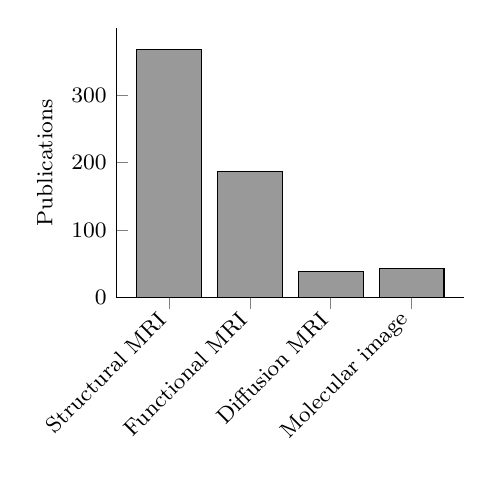
\begin{tikzpicture}
            \begin{axis}[
                ybar,
                height=5cm,
                width=6cm,
                bar width=0.8,
                xmin=0.35,
                xmax=4.65,
                ymin=0,
                xtick={1, 2, 3, 4},
                xticklabels={Structural MRI, Functional MRI, Diffusion MRI, Molecular image},
                x tick label style={
                    rotate=45,anchor=east,
                    font=\footnotesize
                },
                tick label style={
                    font=\footnotesize
                },
                ylabel={\footnotesize{Publications}},
                ymax=399,
                axis y line*=left,
                axis x line*=bottom,
                xtick align=outside
            ]
                \addplot[fill=gray!80] coordinates {
                    (1, 367)
                    (2, 186)
                    (3, 39)
                    (4, 43)
                };
            \end{axis}
        \end{tikzpicture}
    }

    \newsavebox{\colouredmodalities}
    \sbox{\colouredmodalities}{%
        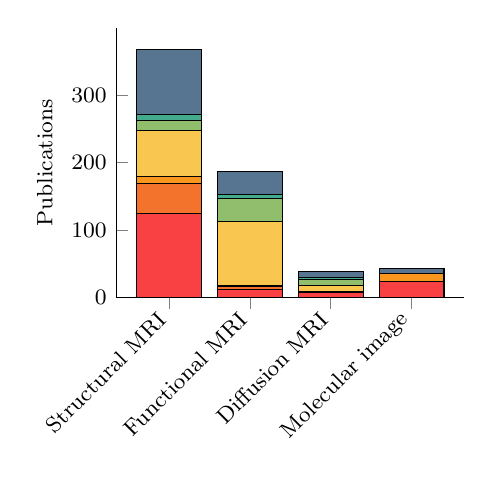
\begin{tikzpicture}
            \begin{axis}[
                ybar stacked,
                height=5cm,
                width=6cm,
                bar width=0.8,
                xmin=0.35,
                xmax=4.65,
                ymin=0,
                xtick={1, 2, 3, 4},
                xticklabels={Structural MRI, Functional MRI, Diffusion MRI, Molecular image},
                x tick label style={
                    rotate=45,anchor=east,
                    font=\footnotesize
                },
                tick label style={
                    font=\footnotesize
                },
                ylabel={\footnotesize{Publications}},
                ymax=399,
                axis y line*=left,
                axis x line*=bottom,
                xtick align=outside
            ]
                \addplot[fill=color1] coordinates {
                    (1, 124)
                    (2, 12)
                    (3, 7)
                    (4, 23)
                };
                \addplot[fill=color2] coordinates {
                    (1, 45)
                    (2, 4)
                    (3, 1)
                    (4, 0)
                };
                \addplot[fill=color3] coordinates {
                    (1, 10)
                    (2, 1)
                    (3, 0)
                    (4, 12)
                };
                \addplot[fill=color4] coordinates {
                    (1, 68)
                    (2, 96)
                    (3, 10)
                    (4, 0)
                };
                \addplot[fill=color5] coordinates {
                    (1, 15)
                    (2, 34)
                    (3, 9)
                    (4, 0)
                };
                \addplot[fill=color6] coordinates {
                    (1, 9)
                    (2, 5)
                    (3, 2)
                    (4, 0)
                };
                \addplot[fill=color7] coordinates {
                    (1, 96)
                    (2, 34)
                    (3, 10)
                    (4, 8)
                };
            \end{axis}
        \end{tikzpicture}
    }

    \newsavebox{\casehippo}
    \sbox{\casehippo}{%
        \begin{tikzpicture}
            \begin{axis}[
                width=4cm,
                height=4cm,
                ymajorticks=false,
                xmin=2491,
                xmax=11269,
                xtick pos=bottom,
                axis x line*=bottom,
                hide y axis,
                ymin=0,
                xtick={4000, 7000, 10000},
                scaled x ticks=false,
                ticklabel style = {font=\scriptsize},
                xlabel={\scriptsize{$mm^3$}},
                x label style={at={(axis description cs:0.5,-0.15)},anchor=north},
                ymax=0.0005,
                clip=false
            ]
                \addplot[name path=zero] coordinates {
                    (2491, 0) (11269, 0)
                };
                \addplot[
                    color1,
                    thick,
                    name path=case
                ] table [
                    x=volume,
                    y=AD,
                    col sep=comma
                ] {data/hippocampus_traces.csv};
                \tikzfillbetween[of=zero and case]{color1, opacity=0.5};
                \node[draw=color1,fill=color1!50, inner sep=2pt,label=right:{\scriptsize{DEM}}] at (axis cs: 10000, 0.0004) {};
            \end{axis}
        \end{tikzpicture}
    }

    \newsavebox{\hippo}
    \sbox{\hippo}{%
        \begin{tikzpicture}
            \begin{axis}[
                width=4cm,
                height=4cm,
                ymajorticks=false,
                xmin=2491,
                xmax=11269,
                xtick pos=bottom,
                axis x line*=bottom,
                hide y axis,
                ymin=0,
                xtick={4000, 7000, 10000},
                scaled x ticks=false,
                ticklabel style = {font=\scriptsize},
                xlabel={\scriptsize{$mm^3$}},
                x label style={at={(axis description cs:0.5,-0.15)},anchor=north},
                ymax=0.0005,
                clip=false
            ]
                \addplot[name path=zero] coordinates {
                    (2491, 0) (11269, 0)
                };
                \addplot[
                    color1,
                    thick,
                    name path=case
                ] table [
                    x=volume,
                    y=AD,
                    col sep=comma
                ] {data/hippocampus_traces.csv};
                \addplot[
                    color6,
                    thick,
                    name path=control
                ] table [
                    x=volume,
                    y=CN,
                    col sep=comma
                ] {data/hippocampus_traces.csv};
                \tikzfillbetween[of=zero and case]{color1, opacity=0.5};
                \tikzfillbetween[of=zero and control]{color6, opacity=0.5};
                \node[draw=color1,fill=color1!50, inner sep=2pt,label=right:{\scriptsize{DEM}}] at (axis cs: 10000, 0.0004) {};
                \node[draw=color6,fill=color6!50, inner sep=2pt,label=right:{\scriptsize{HC}}] at (axis cs: 10000, 0.00035) {};
            \end{axis}
        \end{tikzpicture}
    }

    \newsavebox{\hippoauc}
    \sbox{\hippoauc}{%
        \begin{tikzpicture}
            \begin{axis}[
                width=4cm,
                height=4cm,
                xmin=0,
                xmax=1,
                ymin=0,
                ymax=1,
                ticklabel style = {font=\scriptsize},
                xtick={0, 0.25, 0.5, 0.75, 1},
                ytick={0, 0.25, 0.5, 0.75, 1},
                xtick pos=bottom,
                ytick pos=left,
                xlabel=\scriptsize{fpr},
                ylabel=\scriptsize{tpr},
                x label style={at={(axis description cs:0.5,-0.15)},anchor=north},
                y label style={at={(axis description cs:-0.25,.5)},anchor=south},
            ]
            \addplot[draw=none, name path=zero] coordinates {
                (0, 0)
                (1, 0)
            };
            \addplot[
                color7,
                very thick,
                name path=roc
            ] table [
                x=fpr,
                y=tpr,
                col sep=comma
            ] {data/hippocampus_roc.csv};
            \tikzfillbetween[of=zero and roc]{color7, opacity=0.75};
            \node[anchor=south east] at (axis cs: 0.97, 0.02) {\textcolor{white}{\scriptsize{accuracy=0.81}}};
            \end{axis}
        \end{tikzpicture}
    }

    \begin{frame}[t]{Background}
        \centering
        \begin{tikzpicture}
            \colorlet{hiddencolour}{black!20}

            \def\labelsize{\scriptsize}

            \node[] at (0, 0) {};
            \node[draw=black] at (-5, 0) {};
            \node[draw=black] at (5, -7) {};
            \onslide<1>{
                \node[align=center] at (0, -0.5) {
                    The role of neuroimaging beyond T1-weighted MRI in the\\diagnosis and prediction of neuropsychiatric disorders
                };
            }
            \only<2-6>{
                \node[align=center] at (0, -0.5) {
                    \textcolor{hiddencolour}{The role of }neuroimaging \textcolor{hiddencolour}{beyond T1-weighted MRI in the}\\\textcolor{hiddencolour}{diagnosis and prediction of neuropsychiatric disorders}
                };
                \onslide<4->{
                    \node[label=below:{\labelsize{Sample from the MNE library}}] at (1.5, -2.5) {
                        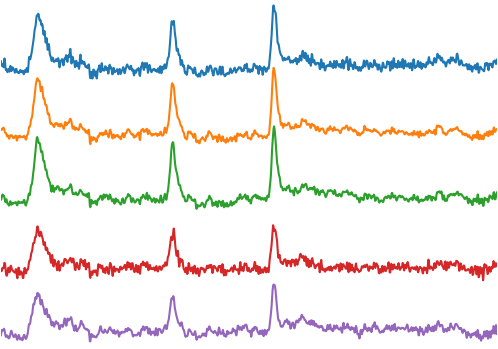
\includegraphics[width=3.75cm]{data/eeg.png}
                    };
                }
                \onslide<5->{
                    %https://www.ncbi.nlm.nih.gov/pmc/articles/PMC4980915/
                    \node[label=below:{\labelsize{Sample from Tremlay et al., 2016}}] at (0.7, -5.1) {
                        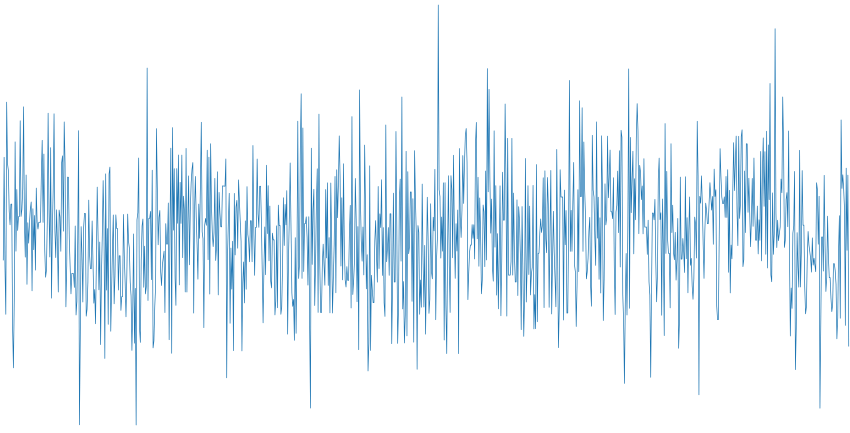
\includegraphics[width=3cm]{data/patch_clamp.png}
                    };
                    \node[font=\tiny, align=center, anchor=south] at (0, -7.75) {
                        Tremblay, R., Lee, S., \& Rudy, B. (2016). GABAergic interneurons in the neocortex: from cellular properties to circuits. Neuron,\\91(2), 260-292
                    };
                }
                \onslide<6->{
                    \node[label=below:{\labelsize{Meta Quest Pro}}] at (3.75, -6.1) {
                        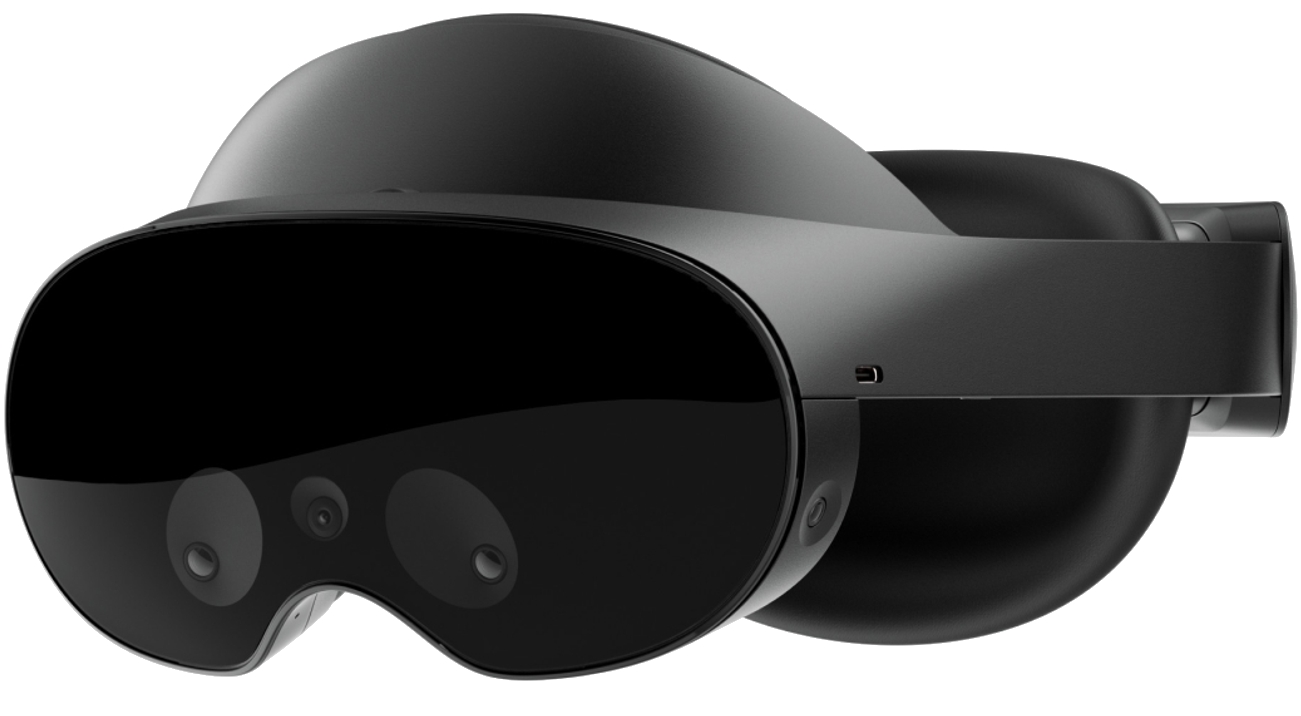
\includegraphics[width=2cm]{data/meta_quest.png}
                    };
                }
            }
            \onslide<3-6,8-12>{
                \node[inner sep=0pt, label=below:{\labelsize{Bert from FreeSurfer 7.3}}] at (-3, -4) {
                    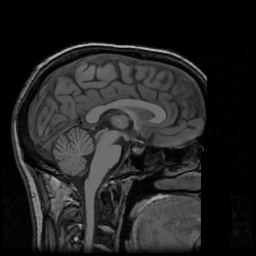
\includegraphics[width=3cm]{data/bert_sagittal.png}
                };
            }
            \only<7-12>{
                \node[align=center] at (0, -0.5) {
                    \textcolor{hiddencolour}{The role of neuroimaging beyond }T1-weighted MRI \textcolor{hiddencolour}{in the}\\\textcolor{hiddencolour}{diagnosis and prediction of neuropsychiatric disorders}
                };
                \only<9>{
                    \node[] at (2, -4.2) {
                        3D
                    };
                }
                \only<10>{
                    \node[] at (2, -4.2) {
                        Saggital, axial
                    };
                }
                \only<11>{
                    \node[] at (2, -4.2) {
                        \usebox{\modalities}
                    };
                }
                \only<12>{
                    \node[] at (2, -4.2) {
                        \usebox{\colouredmodalities}
                    };
                }
            }
            \only<13-15>{
                \def\nodefont{\footnotesize}
                \node[align=center] at (0, -0.5) {
                    \textcolor{hiddencolour}{The role of neuroimaging beyond T1-weighted MRI in the}\\\textcolor{hiddencolour}{diagnosis and prediction of }neuropsychiatric disorders
                };
                \onslide<14->{
                    \node[align=center, font=\nodefont] at (-2, -2) {
                        Alzheimer's disease (AD) and other\\causes of dementia (DEM)
                    };
                    \node[align=center, font=\nodefont] at (-2.8, -2.8) {
                        Multiple Sclerosis (MS)
                    };
                    \node[align=center, font=\nodefont] at (-1.3, -3.2) {
                        Parkinson's Disease (PD)
                    };
                }

                \onslide<15->{
                    \node[align=center, font=\nodefont] at (1.9, -2.2) {
                        Bipolar Disorder (BP)
                    };
                    \node[align=center, font=\nodefont] at (1.6, -2.6) {
                        Schizophrenia (SCZ)
                    };
                    \node[align=center, font=\nodefont] at (2.8, -3.3) {
                        Depressive disorders, including\\major depressive disorder (MDD)
                    };
                }
            }
            \onslide<16->{
                \node[align=center] at (0, -0.5) {
                    \textcolor{hiddencolour}{The role of neuroimaging beyond T1-weighted MRI in the}\\diagnosis and prediction \textcolor{hiddencolour}{of neuropsychiatric disorders}
                };
                \only<17>{
                    \node[label=below:{\scriptsize{Generated by DALL-E 3}}] at (0, -4.2) {
                        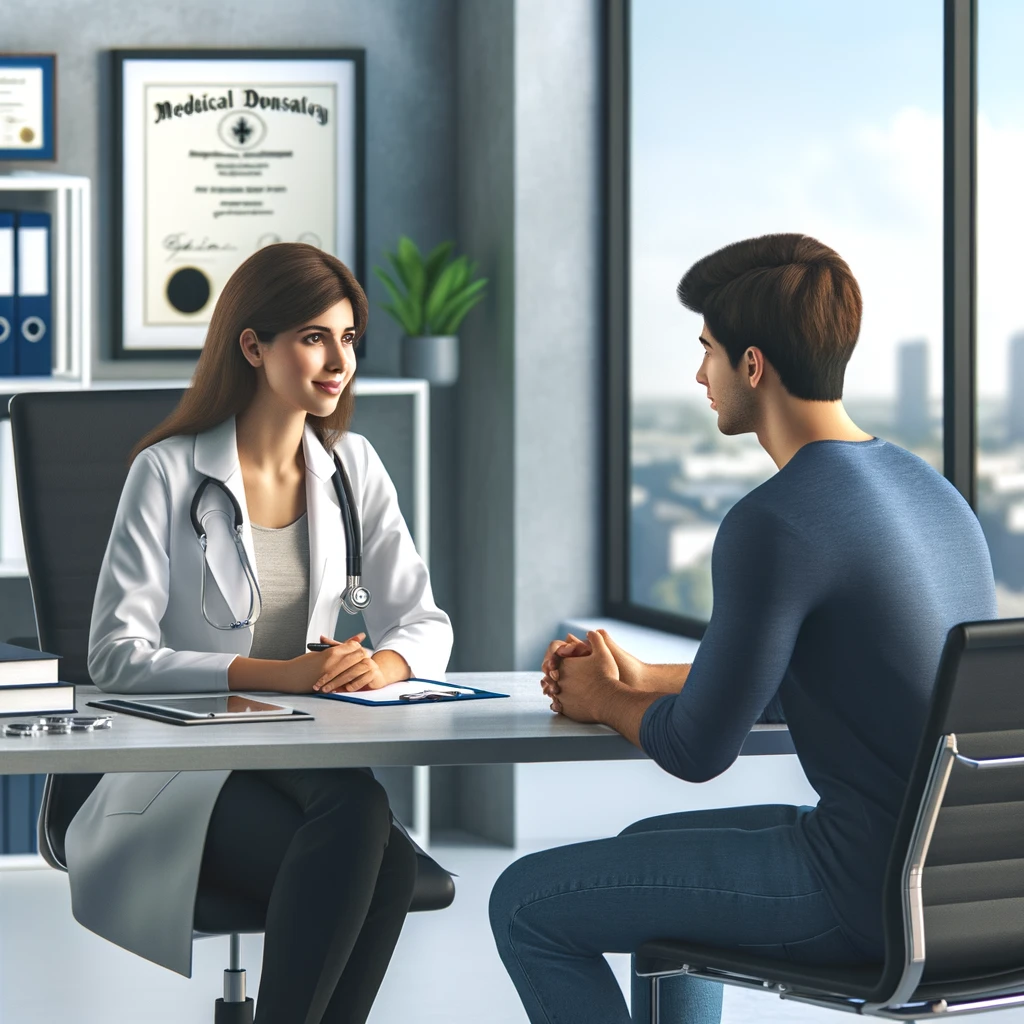
\includegraphics[width=5cm]{data/medical_consultancy.png}
                    };
                };
                \only<18>{
                    \node[label=below:{\labelsize{Vogel \& Black (2024)}}, inner sep=0pt, draw=black] at (0, -3.5) {
                        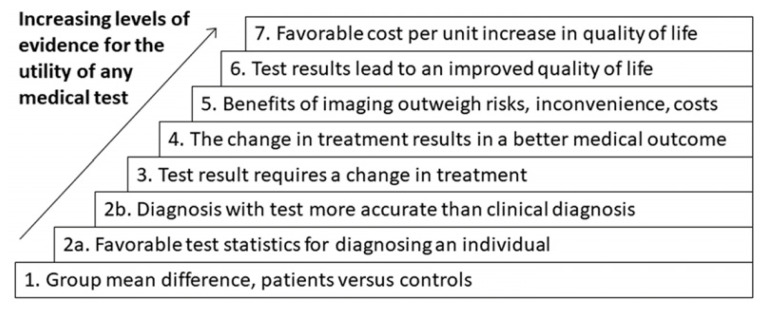
\includegraphics[width=7cm]{data/diagnostic_predictions.jpeg}
                    };

                    \node[font=\tiny, anchor=south,align=center, inner sep=1pt] (psych-citation) at (0, -7.65) {
                        Vogel, A. C., \& Black, K. J. (2024). Brain Imaging in Routine Psychiatric Practice. Missouri Medicine, 121(1), 37
                    };

                }
                \onslide<19->{
                    \only<19,24-25>{
                        \node[inner sep=0pt] (bert) at (-2.8, -4)  {
                            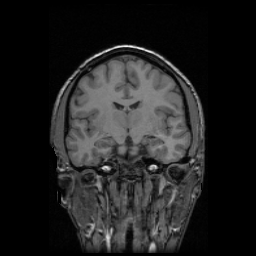
\includegraphics[width=3.5cm]{data/bert_coronal.png}
                        };
                    }
                    \onslide<20-23>{
                        \node[inner sep=0pt] (bert) at (-2.8, -4) {
                            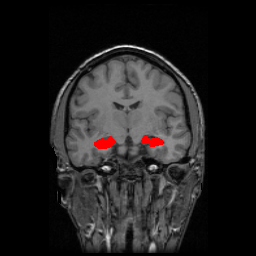
\includegraphics[width=3.5cm]{data/bert_coronal_marked.png}
                        };
                    }
                    \only<21-22>{
                        \node[] at (3.4, -4.3) {
                            \scriptsize{Data from ADNI}
                        };
                        \node[font=\tiny, align=center, anchor=south] at (0, -7.75) {
                            Jack Jr, C. R., Bernstein, M. A., Fox, N. C., Thompson, P., Alexander, G., Harvey, D., ... \& Weiner, M. W. (2008). The Alzheimer's disease\\neuroimaging initiative (ADNI): MRI methods. Journal of Magnetic Resonance Imaging: An Official Journal of the International\\Society for Magnetic Resonance in Medicine, 27(4), 685-691
                        };
                    }
                    \only<21>{
                        \node[anchor=south] at (3.3, -4.15) {
                            \usebox{\casehippo}
                        };
                    }
                    \only<22,23>{
                        \node[anchor=south] at (3.3, -4.15) {
                            \usebox{\hippo}
                        };
                    }
                    \only<23>{
                        \node[] at (2.67, -5.5) {
                            \usebox{\hippoauc}
                        };
                    }
                    \onslide<24->{
                        \node[align=center,draw=gray,fill=gray!20, inner sep=5pt] (model) at (1.2, -4) {Predictive\\model};
                        \node[align=center,text depth=0, anchor=west] (patient) at (3.3, -3.6) {Patient};
                        \node[align=center,text depth=0, anchor=west] (control) at (3.3, -4.4) {Control};

                        \draw[-stealth, thick] (bert) -- (model);
                        \draw[-stealth, thick] (model.east) -- (patient.west);
                        \draw[-stealth, thick] (model.east) -- (control.west);
                    }
                    \only<25>{
                        \node[font=\small] at (1.5, -6) {
                            $\mathrm{accuracy}=\frac{\mathrm{correct\ predictions}}{\mathrm{all\ predictions}}$
                        };
                    }
                }
            }
        \end{tikzpicture}
    \end{frame}
    % \section{\large{Neuroimaging modalities for diagnostic predictions}}

    % \begin{frame}{Approach}
    %     \begin{tikzpicture}
    %         \node[anchor=east] at (0, 0) {
    %             Non-T1 structural MRI
    %         };
    %         \node[anchor=east] at (0, -0.75) {
    %             Diffusion MRI
    %         };
    %         \node[anchor=east] at (0, -1.5) {
    %             Functional MRI
    %         };
    %         \node[anchor=east] at (0, -2.25) {
    %             Molecular imaging
    %         };

    %         \onslide<2->{
    %             \node[anchor=east,rotate=45] at (1, -2.75) {Dementia};
    %             \node[anchor=east,rotate=45] at (2, -2.75) {Multiple sclerosis};
    %             \node[anchor=east,rotate=45] at (3, -2.75) {Parkinson's disease};
    %             \node[anchor=east,rotate=45] at (4, -2.75) {Schizophrenia};
    %             \node[anchor=east,rotate=45] at (5, -2.75) {Major depressive disorder};
    %             \node[anchor=east,rotate=45] at (6, -2.75) {Bipolar disorder};
    %         }

    %         \onslide<3->{
    %             \draw[] (0.5, 0.375) -- (0.5, -2.625);
    %             \draw[] (1.5, 0.375) -- (1.5, -2.625);
    %             \draw[] (2.5, 0.375) -- (2.5, -2.625);
    %             \draw[] (3.5, 0.375) -- (3.5, -2.625);
    %             \draw[] (4.5, 0.375) -- (4.5, -2.625);
    %             \draw[] (5.5, 0.375) -- (5.5, -2.625);
    %             \draw[] (6.5, 0.375) -- (6.5, -2.625);

    %             \draw[] (0.5, 0.375) -- (6.5, 0.375);
    %             \draw[] (0.5, -0.375) -- (6.5, -0.375);
    %             \draw[] (0.5, -1.125) -- (6.5, -1.125);
    %             \draw[] (0.5, -1.875) -- (6.5, -1.875);
    %             \draw[] (0.5, -2.625) -- (6.5, -2.625);
    %         }
    %     \end{tikzpicture}
    % \end{frame}

    % \begin{frame}{Data}
    %     \begin{tikzpicture}
    %         \node[draw=black] at (0, 0) {};
    %         \node[draw=black] at (10, -7) {};

    %         \only<1-4>{
    %             \onslide<1->{
    %                 \node[draw=black,inner sep=2pt] (wolfers) at (2, -1.8) {
    %                     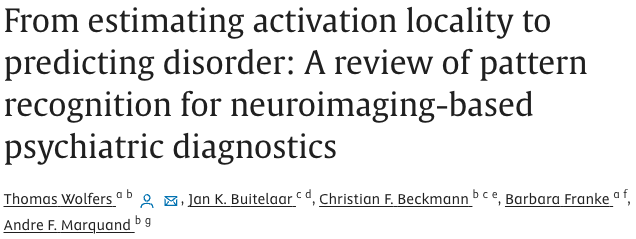
\includegraphics[width=4cm]{data/wolfers_2015.png}
    %                 };
    %             }
    %             \onslide<2->{
    %                 \node[draw=black,inner sep=2pt, anchor=north] (arbabshirani) at ($ (wolfers.south) - (0, 0.2) $) {
    %                     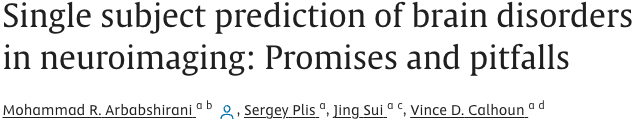
\includegraphics[width=4cm]{data/arbabshirani_2017.png}
    %                 };
    %             }
    %             \onslide<3->{
    %                 \node[draw=black,inner sep=2pt, anchor=north] (rashid) at ($ (arbabshirani.south) - (0, 0.2) $) {
    %                     
\includegraphics[width=4cm]{data/rashid_2020.png}
    %                 };
    %             }
    %             \onslide<4->{
    %                 \node[draw=black,inner sep=2pt, anchor=north] (quaak) at ($ (rashid.south) - (0, 0.2) $) {
    %                     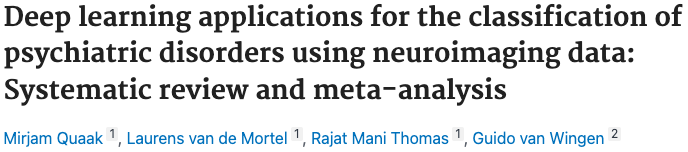
\includegraphics[width=4cm]{data/quaak_2021.png}
    %                 };
    %             }
    %         }
    %         \only<5>{
    %             \node[draw=black,inner sep=2pt] (ebrahim) at (2, -2.2) {
    %                 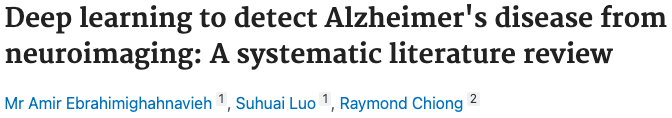
\includegraphics[width=4cm]{data/ebrahimighahnavieh_2020.png}
    %             };
    %             \node[draw=black,inner sep=2pt, anchor=north] (mirzaei) at ($ (ebrahim.south) - (0, 0.2) $) {
    %                 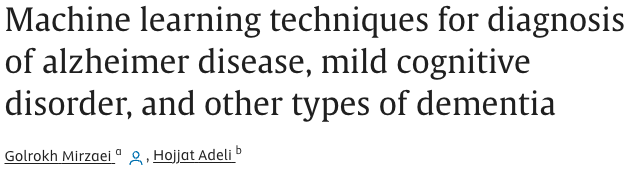
\includegraphics[width=4cm]{data/mirzaei_2022.png}
    %             };

    %             \node[draw=black,inner sep=2pt, anchor=north] (fathi) at ($ (mirzaei.south) - (0, 0.2) $) {
    %                 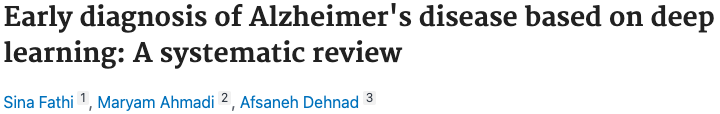
\includegraphics[width=4cm]{data/fathi_2022.png}
    %             };
    %         }
    %         \only<6>{
    %             \node[draw=black,inner sep=2pt] (shoeibi) at (2, -2.8) {
    %                 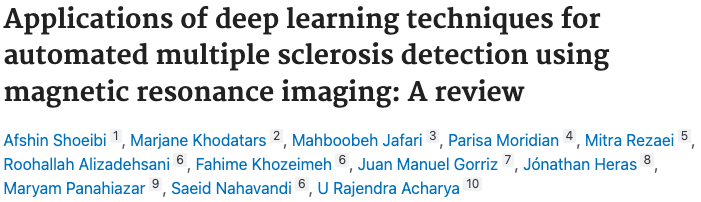
\includegraphics[width=4cm]{data/shoeibi_2021.png}
    %             };
    %             \node[draw=black,inner sep=2pt, anchor=north] (aslam) at ($ (shoeibi.south) - (0, 0.2) $) {
    %                 
\includegraphics[width=4cm]{data/aslam_2022.png}
    %             };
    %         }
    %         \only<7>{
    %             \node[draw=black,inner sep=2pt] (aggarwal) at (2, -3.5) {
    %                 
\includegraphics[width=4cm]{data/aggarwal_2023.png}
    %             };
    %         }
    %         \only<8>{
    %             \node[draw=black,inner sep=2pt] (filippis) at (2, -2.8) {
    %                 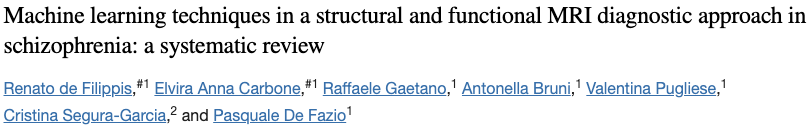
\includegraphics[width=4cm]{data/filippis_2019.png}
    %             };
    %             \node[draw=black,inner sep=2pt, anchor=north] (verma) at ($ (filippis.south) - (0, 0.2) $) {
    %                 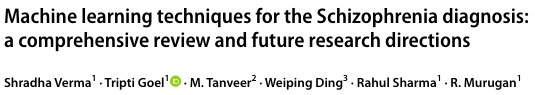
\includegraphics[width=4cm]{data/verma_2023.png}
    %             };

    %         }
    %         \only<9>{
    %             \node[draw=black,inner sep=2pt] (aggarwal) at (2, -3.5) {
    %                 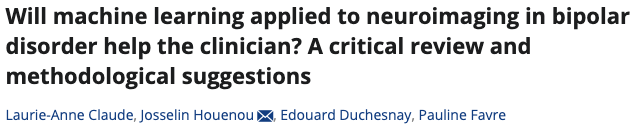
\includegraphics[width=4cm]{data/claude_2020.png}
    %             };
    %             % \node[] at (7.5, -2) {
    %             %     \usebox{\claudedisorders}
    %             % };
    %         }
    %     \end{tikzpicture}
    % \end{frame}

    % \newcommand{\modalityplot}[5]{
    %     \begin{tikzpicture}
    %         \begin{axis}[
    %             ymin=50,
    %             ymax=100,
    %             xtick=#2,
    %             xticklabels=#2,
    %             xlabel=\footnotesize{Year},
    %             ylabel=\footnotesize{Accuracy},
    %             width=4.5cm,
    %             height=4.5cm,
    %             every tick label/.append style={font=\footnotesize},
    %             xtick pos=bottom,
    %             ytick pos=left,
    %             clip=false,
    %             xmin=#3,
    %             xmax=#4
    %         ]
    %             \addplot[
    %                 only marks,
    %                 scatter,
    %                 scatter/classes={
    %                     DEM={mark=*,dem},
    %                     MS={mark=*,ms},
    %                     PD={mark=*,pd},
    %                     SCZ={mark=*,scz},
    %                     MDD={mark=*,mdd},
    %                     BP={mark=*,bp}
    %                 },
    %                 scatter src=explicit symbolic,
    %                 visualization depends on={ln(\thisrow{sample}*0.5) \as \perpointmarksize},
    %                 scatter/@pre marker code/.append style={
    %                     /tikz/mark size=\perpointmarksize
    %                 },
    %                 opacity=0.75
    %             ] table [
    %                 x=year,
    %                 y=accuracy,
    %                 col sep=comma,
    %                 meta=diagnosis
    %             ] {data/#1};
    %             #5
    %         \end{axis}
    %     \end{tikzpicture}
    % }

    % \newsavebox{\ttwostudies}
    % \sbox{\ttwostudies}{%
    %     \modalityplot{t2_studies.csv}{{2016, 2018, 2020, 2022}}{2015.5}{2022.5}{
    %         \node[circle,anchor=south west, draw=pd, fill=pd!75,inner sep=2pt,label=right:{\footnotesize{PD (4)}}] at (axis cs: 2023, 51) {};
    %         \node[circle,anchor=south west, draw=ms, fill=ms!75,inner sep=2pt,label=right:{\footnotesize{MS (11)}}] at (axis cs: 2023, 56) {};
    %     }
    % }

    % \newcommand{\disordermodalityplot}[7]{
    %     \begin{tikzpicture}
    %         \begin{axis}[
    %             ymin=50,
    %             ymax=100,
    %             xlabel=\footnotesize{Sample size},
    %             ylabel=\footnotesize{Accuracy},
    %             height=6cm,
    %             width=8cm,
    %             every tick label/.append style={font=\footnotesize},
    %             xmin=0,
    %             xmax=#5,
    %             xtick pos=bottom,
    %             ytick pos=left,
    %             title={#1 classification studies using #2}
    %         ]
    %             \addplot[
    %                 only marks,
    %                 discard if not={diagnosis}{#1},
    %                 mark=*,
    %                 #6,
    %                 opacity=0.75,
    %                 mark size=3pt
    %             ] table [
    %                 x=sample,
    %                 y=accuracy,
    %                 col sep=comma,
    %             ] {data/#3};
    %             \addplot[
    %                 dashed,
    %                 #6
    %             ] coordinates {
    %                 (0, #4)
    %                 (#5, #4)
    %             };
    %             \node[anchor=north east, #6] at (axis cs: #7, #4) {\footnotesize{#4\%}};
    %         \end{axis}
    %     \end{tikzpicture}
    % }

    % \newsavebox{\msflair}
    % \sbox{\msflair}{%
    %     \disordermodalityplot{MS}{T2/FLAIR}{t2_studies.csv}{90.54}{1200}{ms}{1200}
    % }

    % \newsavebox{\pdflair}
    % \sbox{\pdflair}{%
    %     \disordermodalityplot{PD}{T2/FLAIR}{t2_studies.csv}{90.97}{550}{pd}{470}
    % }

    % \begin{frame}[t]{Other structural MRI modalities}
    %     \only<1-13>{
    %         \begin{tikzpicture}
    %             \def\labelsize{\footnotesize}

    %             \node[draw=black] at (0, 0) {};
    %             \node[draw=black] at (10, -7) {};
    %             \only<1-4>{
    %                 \node[font=\tiny, anchor=south,align=center, inner sep=1pt] (ms-citation) at (5, -7.65) {
    %                     Preson D. C., (2006), MRI Basics, https://case.edu/med/neurology/NR/MRI\%20Basics
    %                 };
    %             }
    %             \only<1-8>{
    %                 \node[anchor=west, inner sep=0pt, outer sep=0pt] (t1) at (0, -3.5) {
    %                     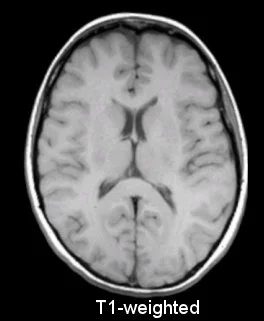
\includegraphics[
    %                         height=1.7cm
    %                     ]{data/t1.png}
    %                 };
    %             }
    %             \only<2-8>{
    %                 \node[anchor=west, inner sep=0pt, outer sep=0pt] (t2) at ($ (t1.east) $) {
    %                     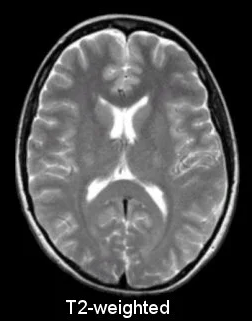
\includegraphics[
    %                         height=1.7cm
    %                     ]{data/t2.png}
    %                 };
    %             }
    %             \only<3>{
    %                 \node[minimum width=0.4cm, minimum height=0.35cm, thick, draw=red] at ($ (t2) + (0, 0.225) $){};
    %                 \node[minimum width=0.4cm, minimum height=0.35cm, thick, draw=red] at ($ (t1) + (0, 0.225) $){};
    %             }
    %             \only<4-8>{
    %                 \node[anchor=west, inner sep=0pt, outer sep=0pt] (flair) at ($ (t2.east) $) {
    %                     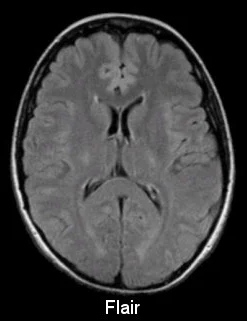
\includegraphics[
    %                         height=1.7cm
    %                     ]{data/flair.png}
    %                 };
    %             }
    %             \only<5>{
    %                 \node[anchor=west] at (5, -3.5) {
    %                     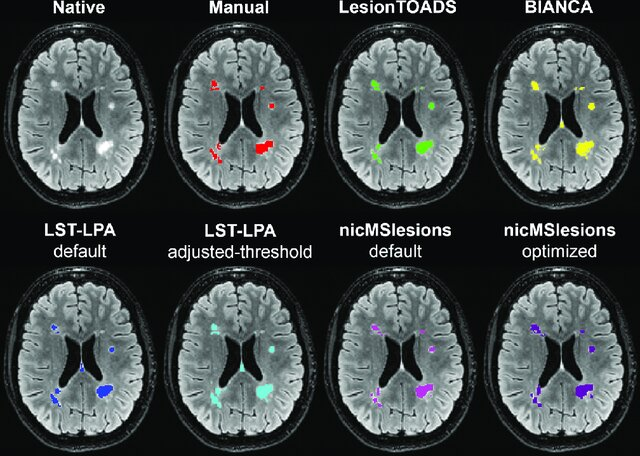
\includegraphics[
    %                         height=3cm,
    %                         trim={0 2.8cm 5.6cm 0.2cm},
    %                         clip
    %                     ]{data/FLAIR_lesion_segmented.jpeg}
    %                 };
    %             }
    %             \only<6>{
    %                 \node[] at (7.1, -3.6) {
    %                     \usebox{\ttwostudies}
    %                 };
    %             };
    %             \only<7>{
    %                 \node[anchor=west] at (5, -3.5) {
    %                     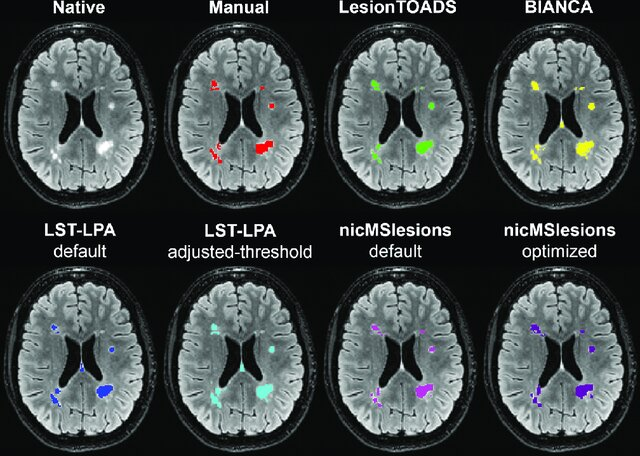
\includegraphics[
    %                         height=3cm,
    %                         trim={0 2.8cm 3.7cm 0.2cm},
    %                         clip
    %                     ]{data/FLAIR_lesion_segmented.jpeg}
    %                 };
    %                 \node[font=\tiny, anchor=south,align=center, inner sep=1pt] (ms-citation) at (5, -7.65) {
    %                     Weeda, M. M., Brouwer, I., de Vos, M. L., de Vries, M. S., Barkhof, F., Pouwels, P. J. W., \& Vrenken, H. (2019). Comparing\\lesion segmentation methods in multiple sclerosis: Input from one manually delineated subject is sufficient for accurate\\lesion segmentation. NeuroImage: Clinical, 24, 102074
    %                 };
    %             }
    %             \only<8>{
    %                 \node[inner sep=0pt, draw=black] at (7.6, -3.2) {
    %                     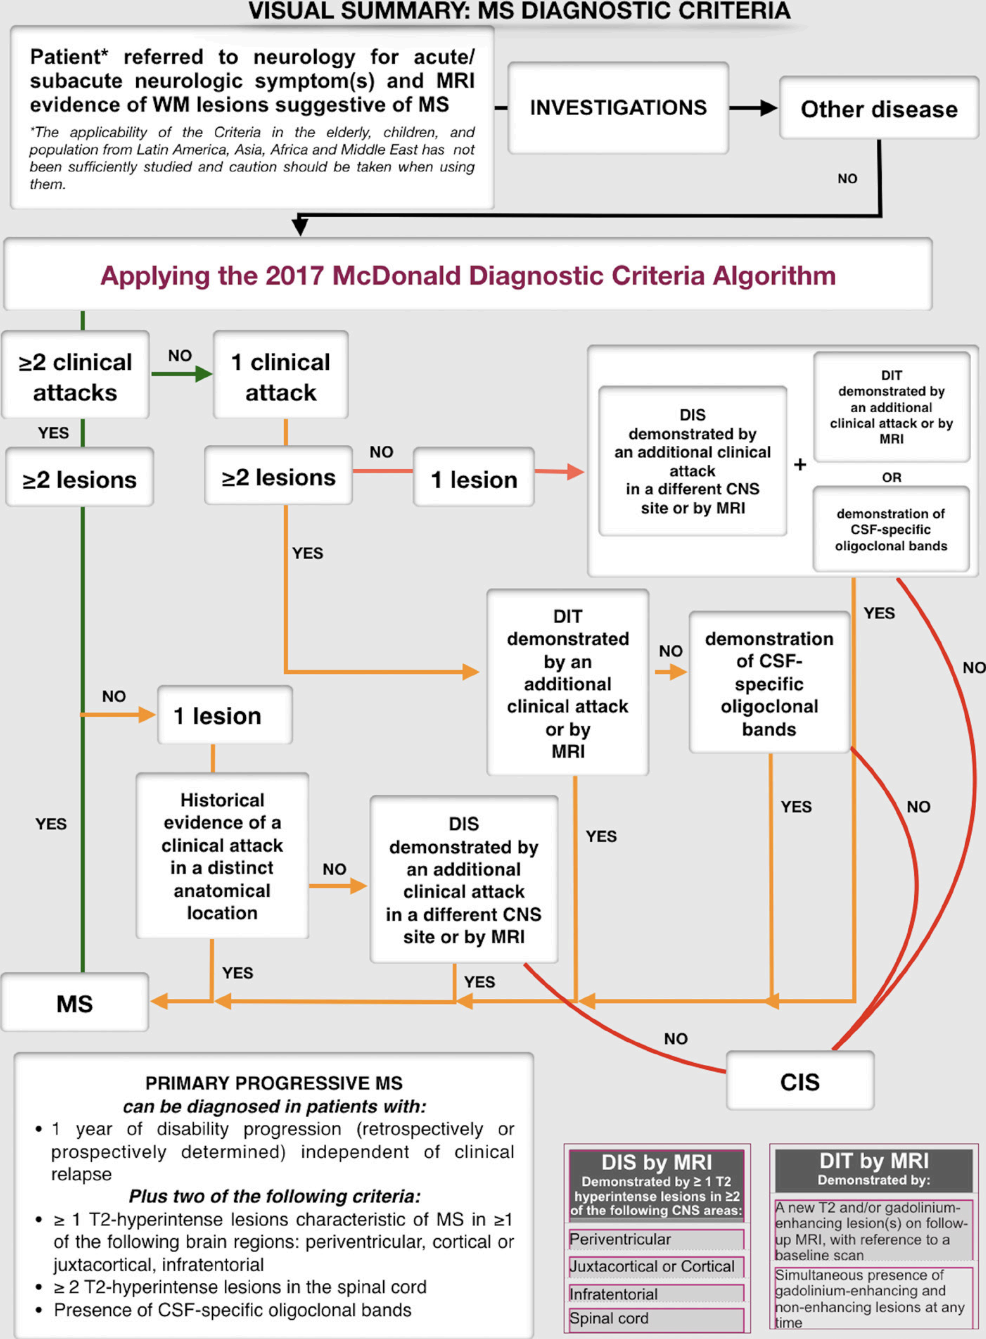
\includegraphics[width=4.5cm]{data/ms_criteria.png}
    %                 };
    %                 \node[font=\tiny, anchor=south,align=center, inner sep=1pt] (ms-citation) at (5, -7.65) {
    %                     De Angelis, F., Brownlee, W. J., Chard, D. T., \& Trip, S. A. (2019). New MS diagnostic criteria in practice. Practical Neurology, 19(1), 64-67
    %                 };
    %             }
    %             \only<9>{
    %                 \node[] at (5, -3.5) {
    %                     \usebox{\msflair}
    %                 };
    %             }
    %             \only<10>{
    %                 \node[inner sep=0pt, draw=black, inner sep=0pt, draw=black] at (5, -3.2) {
    %                     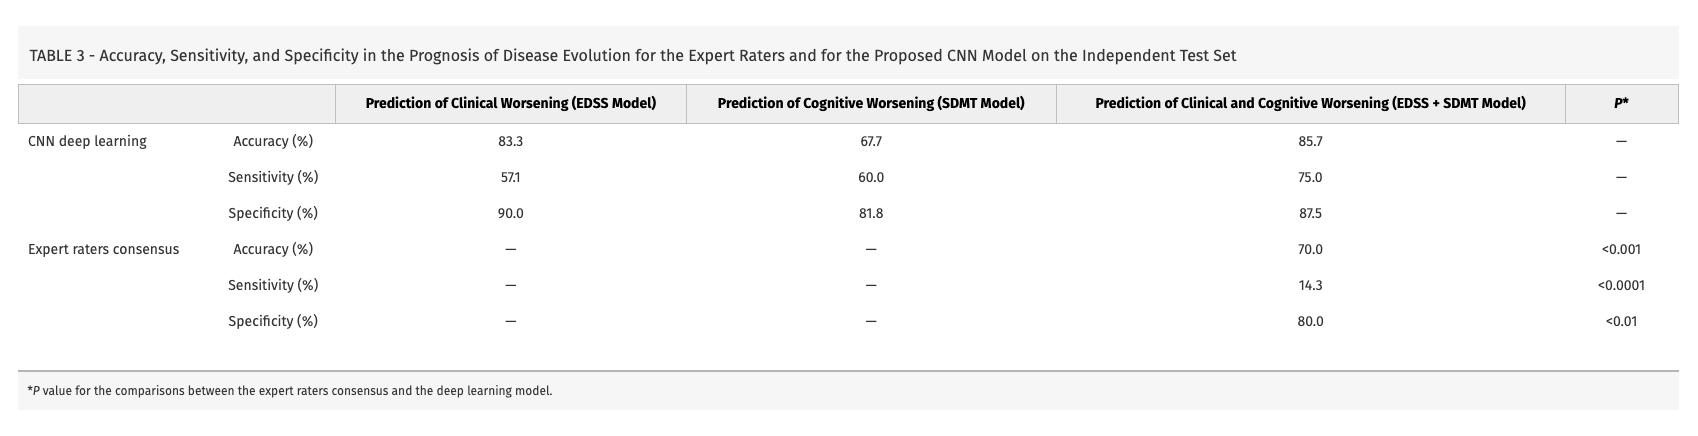
\includegraphics[width=9cm]{data/ms_human_vs_machine.png}
    %                 };
    %                 \node[font=\tiny, anchor=south,align=center, inner sep=1pt] (ms-citation) at (5, -7.65) {
    %                     Storelli, L., Azzimonti, M., Gueye, M., Vizzino, C., Preziosa, P., Tedeschi, G., ... \& Rocca, M. A. (2022). A deep learning approach\\to predicting disease progression in multiple sclerosis using magnetic resonance imaging. Investigative Radiology, 57(7), 423-432
    %                 };
    %             }
    %             \only<11>{
    %                 \node[] at (5, -3.5) {
    %                     \usebox{\pdflair}
    %                 };
    %             }
    %             \only<12-13>{
    %                 \node[font=\tiny, anchor=south,align=center, inner sep=1pt] (ms-citation) at (5, -7.65) {
    %                     Talai, A. S., Sedlacik, J., Boelmans, K., \& Forkert, N. D. (2021). Utility of multi-modal MRI for differentiating of Parkinson's\\disease and progressive supranuclear palsy using machine learning. Frontiers in Neurology, 12, 648548
    %                 };
    %                 \only<12>{
    %                     \node[] at (5, -3.2) {
    %                         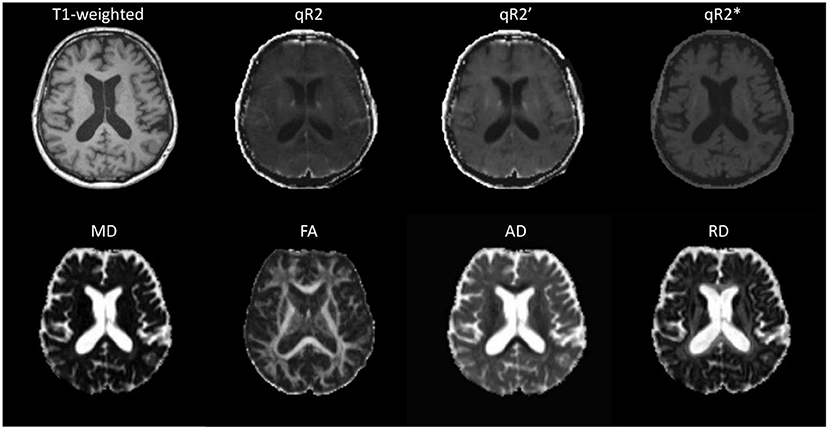
\includegraphics[
    %                             width=8cm,
    %                             trim={0, 8cm, 0, 0},
    %                             clip
    %                         ]{data/pd_t2_r2.jpeg}
    %                     };
    %                 }
    %                 \only<13>{
    %                     \node[inner sep=0pt, draw=black] at (5, -3.2) {
    %                         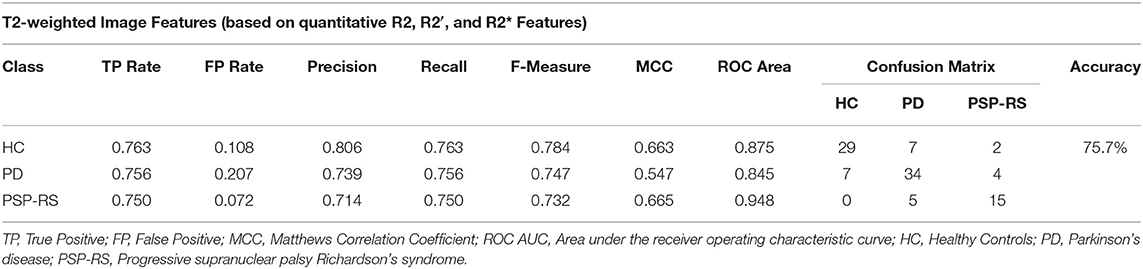
\includegraphics[width=9cm]{data/pd_t2_accuracy.jpeg}
    %                     };
    %                 }
    %             }
    %         \end{tikzpicture}
    %     }
    %     \only<14>{
    %         \begin{itemize}
    %             \setlength\itemsep{-0.3em}
    %             \item \footnotesize{Non-T1 weighted structural MRI}
    %             \begin{itemize}
    %                 \item \scriptsize{High accuracies for classifying MS and PD (>90\%).}
    %                 \item \scriptsize{T2-weighted images used by Storelli et al. for predicting MS prognosis.}
    %                 \item \scriptsize{T2-weighted images used by Talai et al. for differential diagnosis of PD and PSP-RS.}
    %             \end{itemize}
    %         \end{itemize}
    %     }
    % \end{frame}

    % \newsavebox{\dmristudies}
    % \sbox{\dmristudies}{%
    %     \modalityplot{dmri_studies.csv}{{2005, 2010, 2015, 2020}}{2005}{2022}{
    %         \node[circle,anchor=south west, draw=ms, fill=ms!75,inner sep=2pt,label=right:{\footnotesize{MS (1)}}] at (axis cs: 2023, 51) {};
    %         \node[circle,anchor=south west, draw=bp, fill=bp!75,inner sep=2pt,label=right:{\footnotesize{BP (2)}}] at (axis cs: 2023, 56) {};
    %         \node[circle,anchor=south west, draw=dem, fill=dem!75,inner sep=2pt,label=right:{\footnotesize{DEM (6)}}] at (axis cs: 2023, 61) {};
    %         \node[circle,anchor=south west, draw=mdd, fill=mdd!75,inner sep=2pt,label=right:{\footnotesize{MDD (9)}}] at (axis cs: 2023, 66) {};
    %         \node[circle,anchor=south west, draw=scz, fill=scz!75,inner sep=2pt,label=right:{\footnotesize{SCZ (10)}}] at (axis cs: 2023, 71) {};
    %     }
    % }

    % \newsavebox{\dmriscz}
    % \sbox{\dmriscz}{%
    %     \disordermodalityplot{SCZ}{dMRI}{dmri_studies.csv}{84.30}{220}{scz}{220}
    % }

    % \newsavebox{\dmridem}
    % \sbox{\dmridem}{%
    %     \disordermodalityplot{DEM}{dMRI}{dmri_studies.csv}{89.56}{850}{dem}{850}
    % }

    % \begin{frame}[t]{Diffusion MRI}
    %     \only<1-13>{
    %         \begin{tikzpicture}
    %             \node[draw=black] at (0, 0) {};
    %             \node[draw=black] at (10, -7) {};

    %             \only<1-3>{
    %                 \node[] at (2, -3.5) {
    %                     Explanation of DTI
    %                 };
    %             }
    %             \only<2>{
    %                 \node[] at (7.6, -3.6) {
    %                     \usebox{\dmristudies}
    %                 };
    %             };
    %             \only<3>{
    %                 \node[] at (7.6, -3.2) {
    %                     Lack of prediction studies
    %                 };
    %             }
    %             \onslide<4-8>{
    %                 \only<4>{
    %                     \node[] at (5, -3.2) {
    %                         \usebox{\dmriscz}
    %                     };
    %                 }
    %                 \onslide<5->{
    %                     \node[font=\tiny, anchor=south,align=center, inner sep=1pt] (ms-citation) at (5, -7.65) {
    %                         Saglam, Y., Oz, A., Yildiz, G., Ermis, C., Kargin, O. A., Arslan, S., \& Karacetin, G. (2023). Can diffusion\\tensor imaging have a diagnostic utility to differentiate early-onset forms of bipolar disorder and schizophrenia:\\A neuroimaging study with explainable machine learning algorithms. Psychiatry Research: Neuroimaging, 335, 111696
    %                     };
    %                 }
    %                 \only<5>{
    %                     \node[inner sep=0pt, draw=black] at (5, -3.2) {
    %                         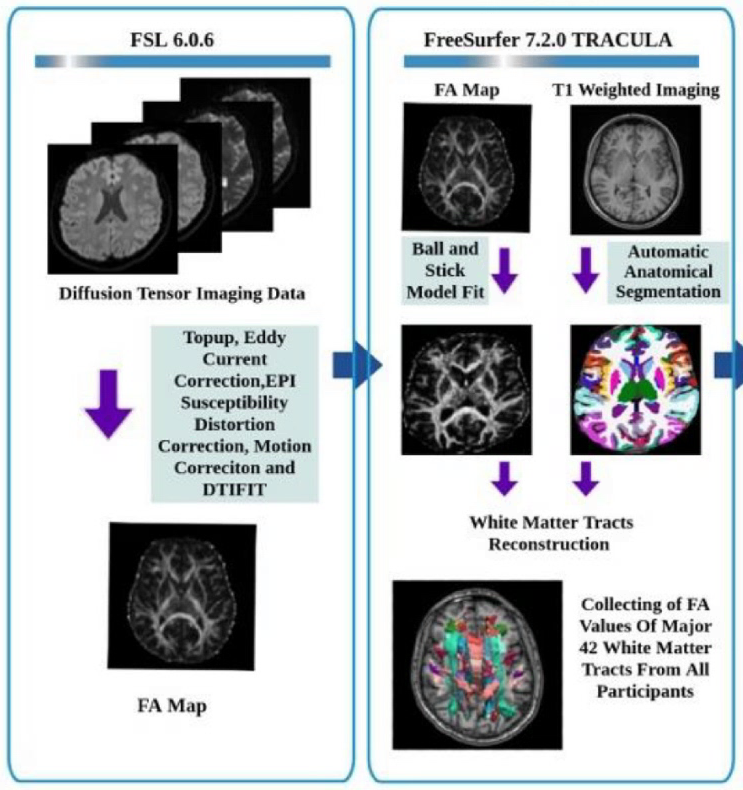
\includegraphics[width=5cm]{data/scz_bp_pipeline.png}
    %                     };
    %                 }
    %                 \only<6>{
    %                     \node[inner sep=0pt, draw=black] at (5, -3.2) {
    %                         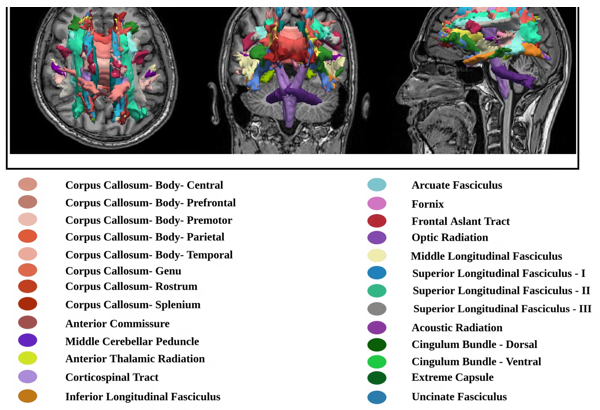
\includegraphics[width=7cm]{data/scz_bp_dti.png}
    %                     };
    %                 }
    %                 \only<7>{
    %                     \node[inner sep=0pt, draw=black] at (5, -3.2) {
    %                         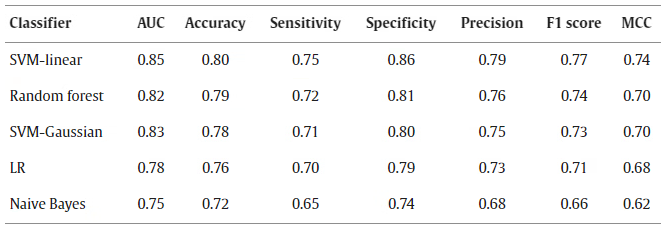
\includegraphics[width=9cm]{data/scz_bp_performance.png}
    %                     };
    %                 }
    %                 \only<8>{
    %                     \node[inner sep=0pt, draw=black] at (5, -3.2) {
    %                         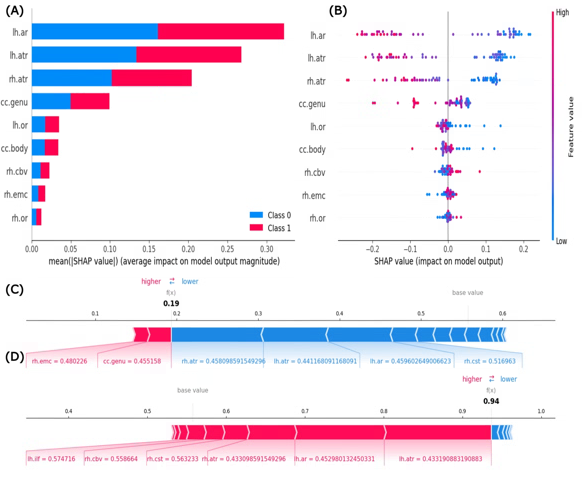
\includegraphics[width=7cm]{data/scz_bp_shap.png}
    %                     };
    %                 }
    %             }

    %             \onslide<9->{
    %                 \only<9>{
    %                     \node[] at (5, -3.2) {
    %                         \usebox{\dmridem}
    %                     };
    %                 }
    %                 \onslide<10->{
    %                     \node[font=\tiny, anchor=south,align=center, inner sep=1pt] (ms-citation) at (5, -7.65) {
    %                             Sun, Y., Bi, Q., Wang, X., Hu, X., Li, H., Li, X., ... \& Han, Y. (2019). Prediction of conversion from amnestic\\mild cognitive impairment to Alzheimer's disease based on the brain structural connectome. Frontiers in neurology, 9, 1178
    %                     };

    %                 }
    %                 \only<10>{
    %                     \node[inner sep=0pt, draw=black] at (5, -3.2) {
    %                         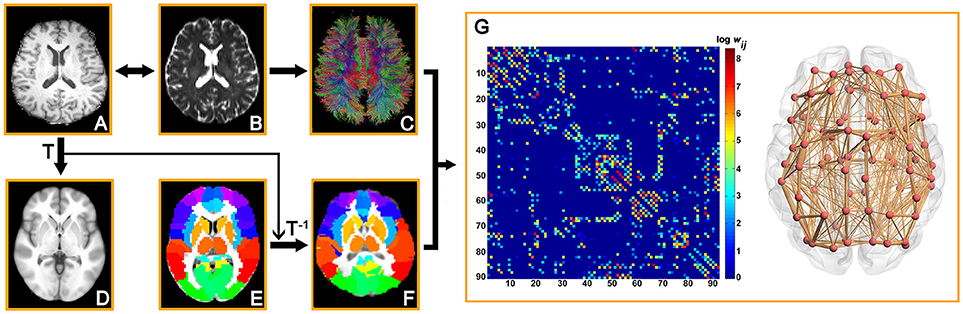
\includegraphics[width=9cm]{data/mci_conversion_overview.jpeg}
    %                     };
    %                 }
    %                 \only<11>{
    %                     \node[inner sep=0pt, draw=black] at (5, -3.2) {
    %                         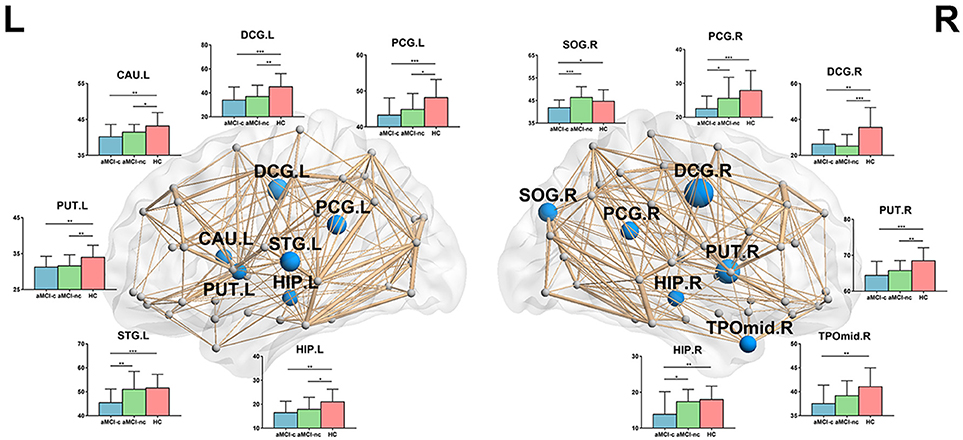
\includegraphics[width=9cm]{data/mci_conversion_hubs.jpeg}
    %                     };
    %                 }
    %                 \only<12-13>{
    %                     \node[inner sep=0pt, draw=black] at (3, -3.2) {
    %                         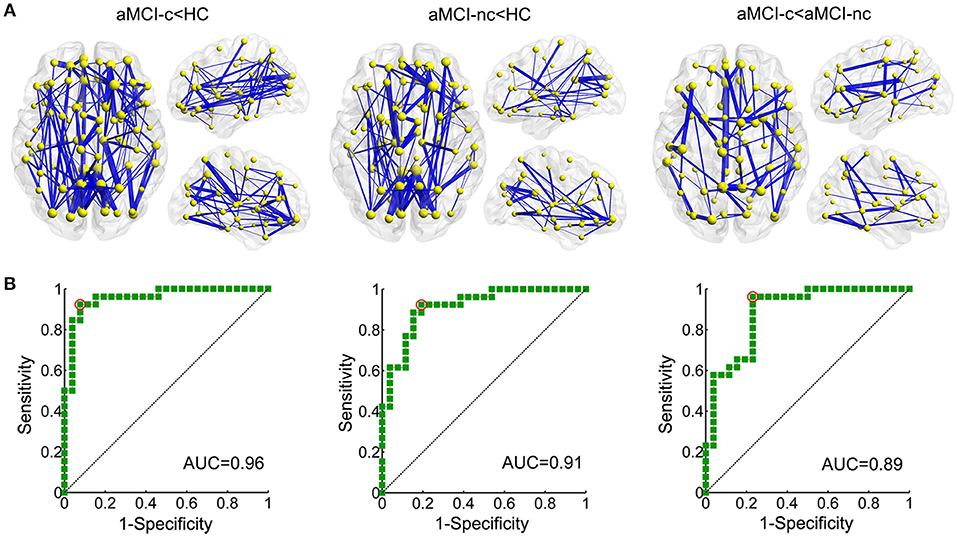
\includegraphics[
    %                             height=5cm,
    %                             trim={22.2cm, 0, 0, 0},
    %                             clip
    %                         ]{data/mci_conversion_connectivity.jpeg}
    %                     };
    %                     \only<13>{
    %                         \node[inner sep=0pt, draw=black] at (7, -3.2) {
    %                             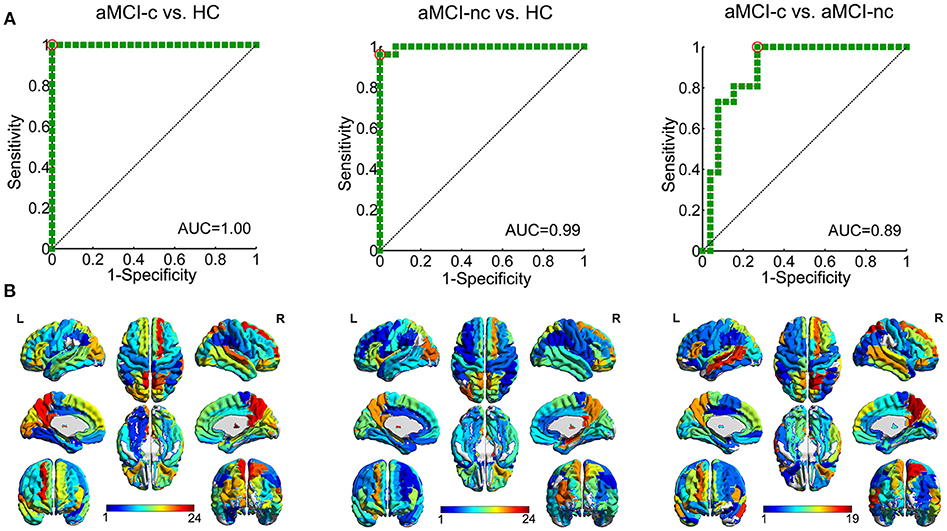
\includegraphics[
    %                                 height=5cm,
    %                                 trim={22.2cm, 0, 0, 0},
    %                                 clip
    %                             ]{data/mci_conversion_regions.jpeg}
    %                         };
    %                     }
    %                 }
    %             }
    %         \end{tikzpicture}
    %     }
    %     \only<14>{
    %         \begin{itemize}
    %             \setlength\itemsep{-0.3em}
    %             \item[\textcolor{gray!50}{\textbullet}] \textcolor{gray!50}{\footnotesize{Non-T1 weighted structural MRI}}
    %             \begin{itemize}
    %                 \item[\textcolor{gray!50}{\textbullet}] \textcolor{gray!50}{\scriptsize{High accuracies for classifying MS and PD (>90\%).}}
    %                 \item[\textcolor{gray!50}{\textbullet}] \textcolor{gray!50}{\scriptsize{T2-weighted images used by Storelli et al. for predicting MS prognosis.}}
    %                 \item[\textcolor{gray!50}{\textbullet}] \textcolor{gray!50}{\scriptsize{T2-weighted images used by Talai et al. for differential diagnosis of PD and PSP-RS.}}
    %             \end{itemize}
    %             \item \footnotesize{Diffusion MRI}
    %             \begin{itemize}
    %                 \item \scriptsize{Few prediction studies, mostly for mental disorders with various accuracies (60-100\%) and DEM (80-100\%)}
    %                 \item \scriptsize{Used by Saglam et al. to differentially diagnose SCZ and BP with 80\% accuracy.}
    %                 \item \scriptsize{Used by Sun et al. to predict conversion from MCI to AD with 81\% accuracy.}
    %             \end{itemize}
    %         \end{itemize}
    %     }
    % \end{frame}

    % \newsavebox{\fmristudies}
    % \sbox{\fmristudies}{%
    %     \modalityplot{fmri_studies.csv}{{2005, 2010, 2015, 2020}}{2005}{2023}{
    %             \node[circle,anchor=south west, draw=pd, fill=pd!75,inner sep=2pt,label=right:{\footnotesize{PD (1)}}] at (axis cs: 2024, 51) {};
    %             \node[circle,anchor=south west, draw=ms, fill=ms!75,inner sep=2pt,label=right:{\footnotesize{MS (4)}}] at (axis cs: 2024, 56) {};
    %             \node[circle,anchor=south west, draw=bp, fill=bp!75,inner sep=2pt,label=right:{\footnotesize{BP (5)}}] at (axis cs: 2024, 61) {};
    %             \node[circle,anchor=south west, draw=dem, fill=dem!75,inner sep=2pt,label=right:{\footnotesize{DEM (12)}}] at (axis cs: 2024, 66) {};
    %             \node[circle,anchor=south west, draw=mdd, fill=mdd!75,inner sep=2pt,label=right:{\footnotesize{MDD (34)}}] at (axis cs: 2024, 71) {};
    %             \node[circle,anchor=south west, draw=scz, fill=scz!75,inner sep=2pt,label=right:{\footnotesize{SCZ (96)}}] at (axis cs: 2024, 76) {};
    %     }
    % }

    % \newsavebox{\mddfmri}
    % \sbox{\mddfmri}{%
    %     \disordermodalityplot{MDD}{fMRI}{fmri_studies.csv}{81.99}{380}{mdd}{380}
    % }

    % \begin{frame}[t]{Functional Magnetic Resonance Imaging (fMRI)}
    %     \only<1-13>{
    %         \begin{tikzpicture}
    %             \node[draw=black] at (0, 0) {};
    %             \node[draw=black] at (10, -7) {};
    %             \only<1-2,4-5>{
    %                 \node[anchor=west] at (1, -3.5) {
    %                     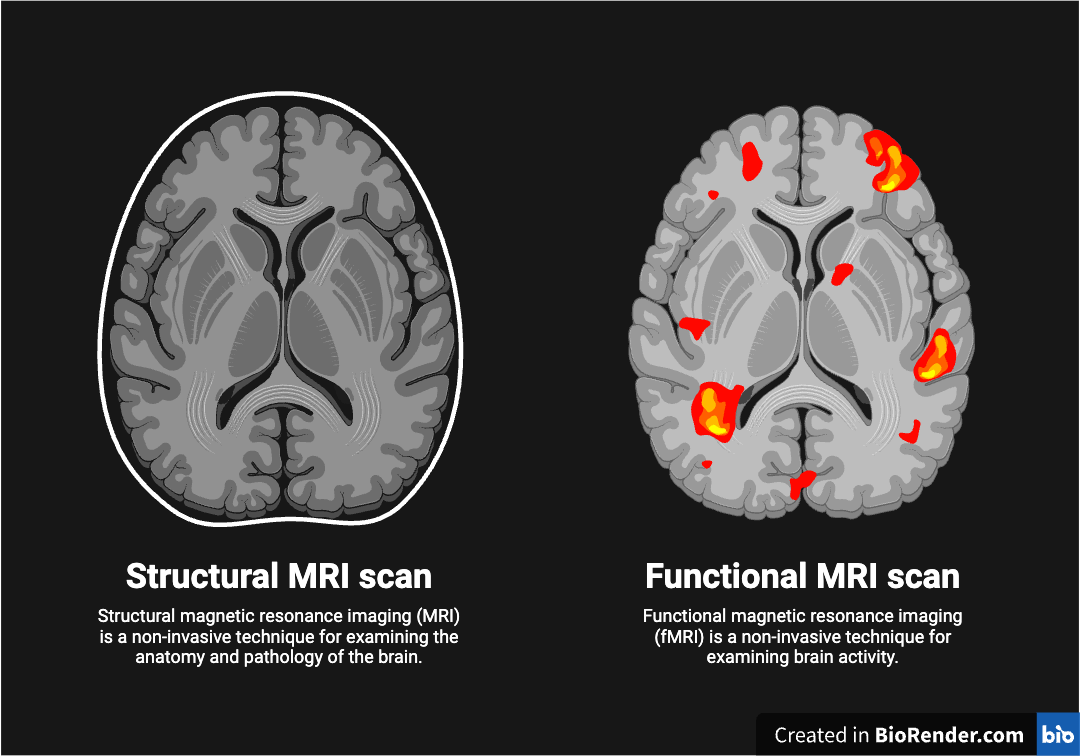
\includegraphics[
    %                         height=3cm,
    %                         trim={75 210 590 70},
    %                         clip
    %                     ]{data/smri_fmri.png}
    %                 };
    %             }
    %             \only<2,4-5>{
    %                 \node[anchor=west] at (1, -3.5) {
    %                     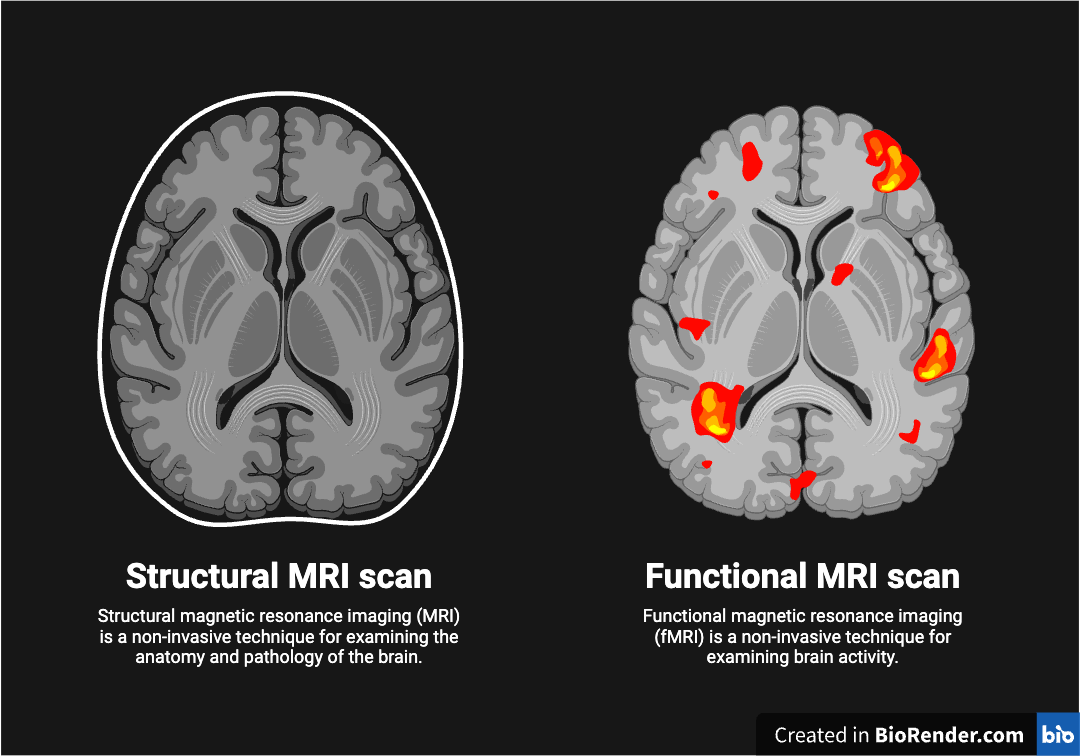
\includegraphics[
    %                         height=3cm,
    %                         trim={595 210 80 70},
    %                         clip
    %                     ]{data/smri_fmri.png}
    %                 };
    %             }
    %             \only<3>{
    %                 \node[anchor=west] at (0, -2.5) {
    %                     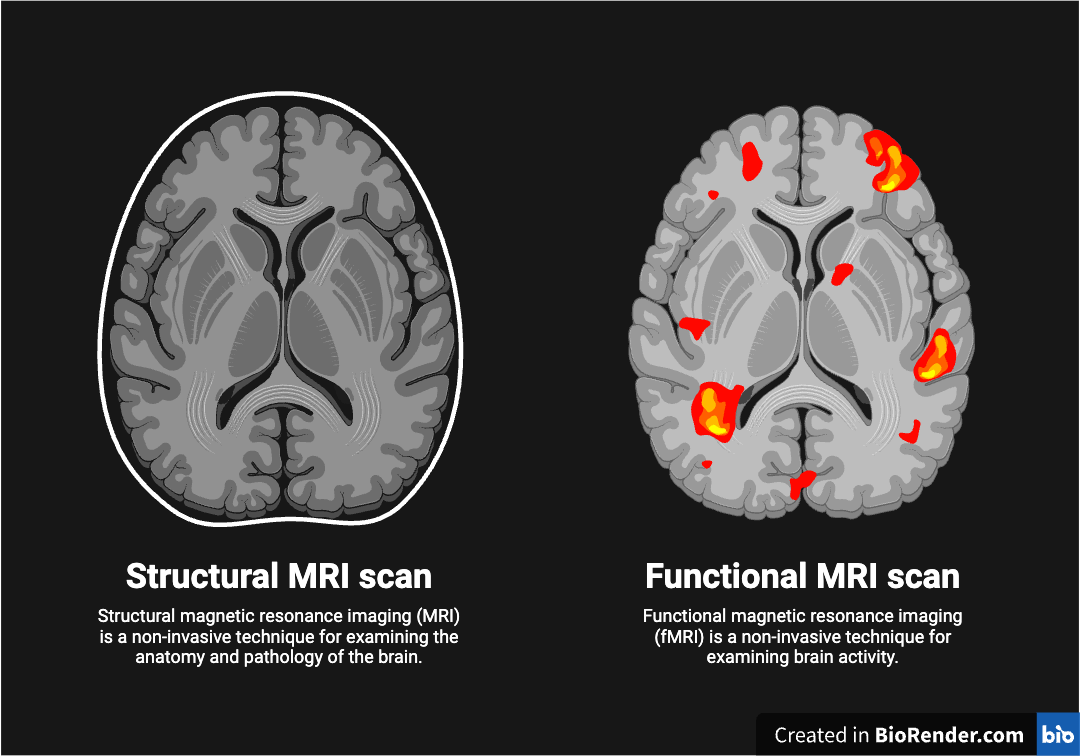
\includegraphics[
    %                         height=3cm,
    %                         trim={75 210 590 70},
    %                         clip
    %                     ]{data/smri_fmri.png}
    %                 };
    %                 \node[anchor=west] (first) at (0, -2.5) {
    %                     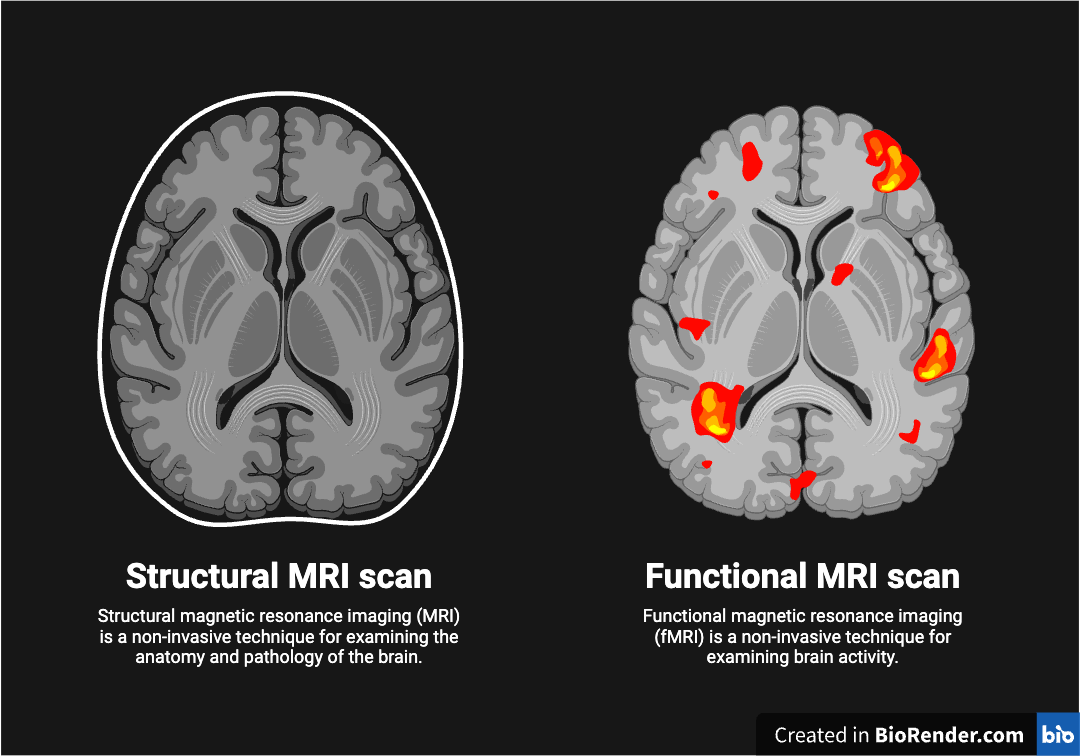
\includegraphics[
    %                         height=3cm,
    %                         trim={595 210 80 70},
    %                         clip
    %                     ]{data/smri_fmri.png}
    %                 };
    %                 \node[anchor=west] at (0.5, -3.0) {
    %                     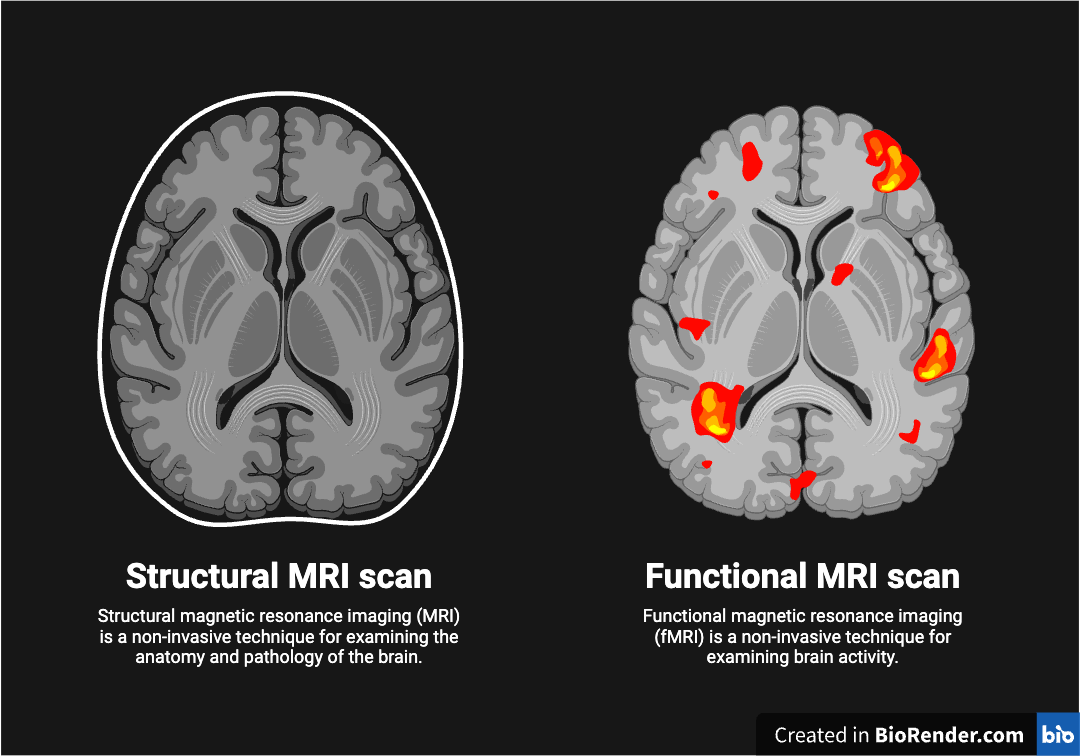
\includegraphics[
    %                         height=3cm,
    %                         trim={75 210 590 70},
    %                         clip
    %                     ]{data/smri_fmri.png}
    %                 };
    %                 \node[anchor=west] at (0.5, -3.0) {
    %                     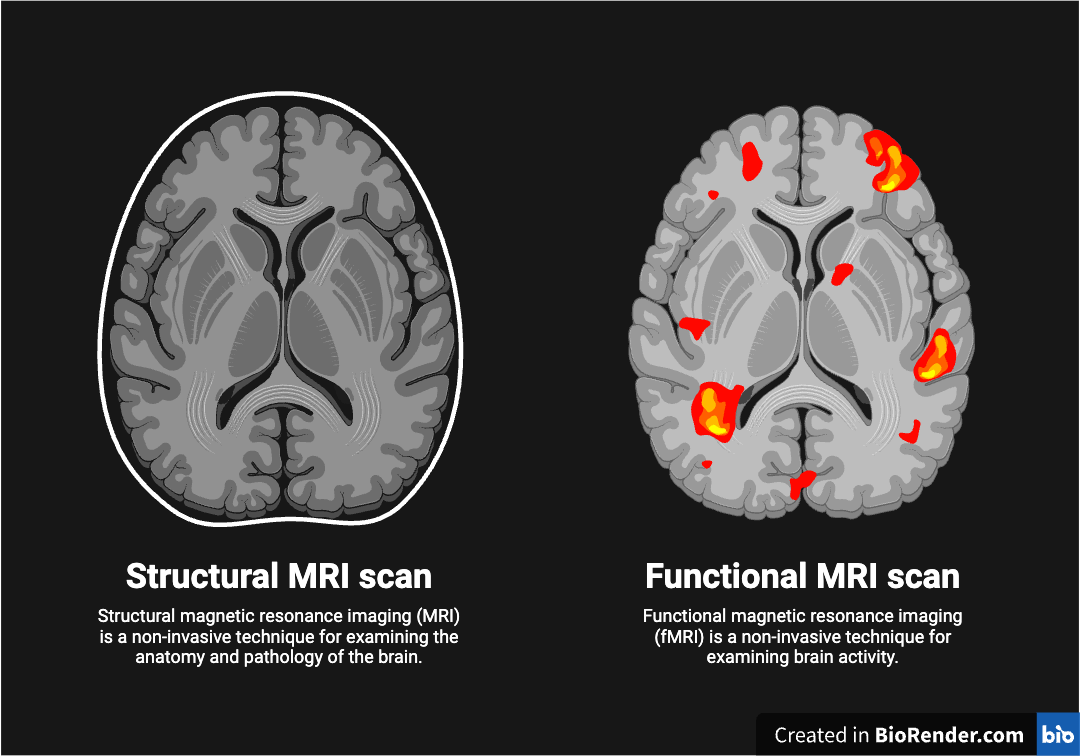
\includegraphics[
    %                         height=3cm,
    %                         trim={595 210 80 70},
    %                         clip
    %                     ]{data/smri_fmri.png}
    %                 };
    %                 \node[anchor=west] at (1, -3.5) {
    %                     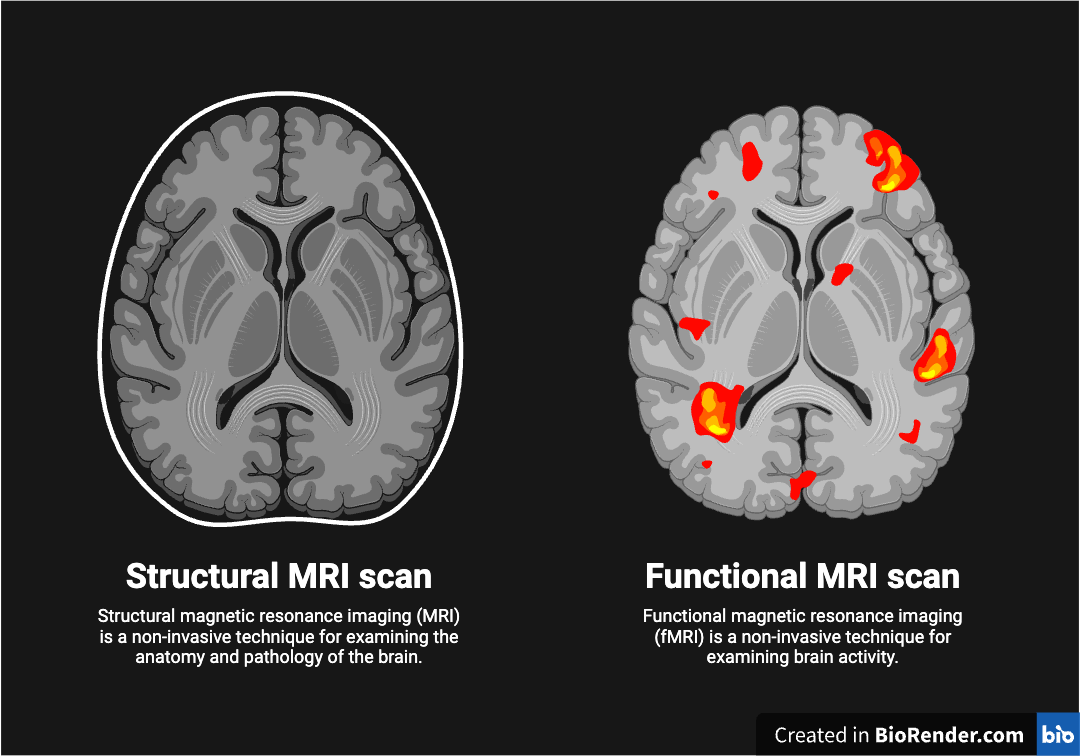
\includegraphics[
    %                         height=3cm,
    %                         trim={75 210 590 70},
    %                         clip
    %                     ]{data/smri_fmri.png}
    %                 };
    %                 \node[anchor=west] at (1, -3.5) {
    %                     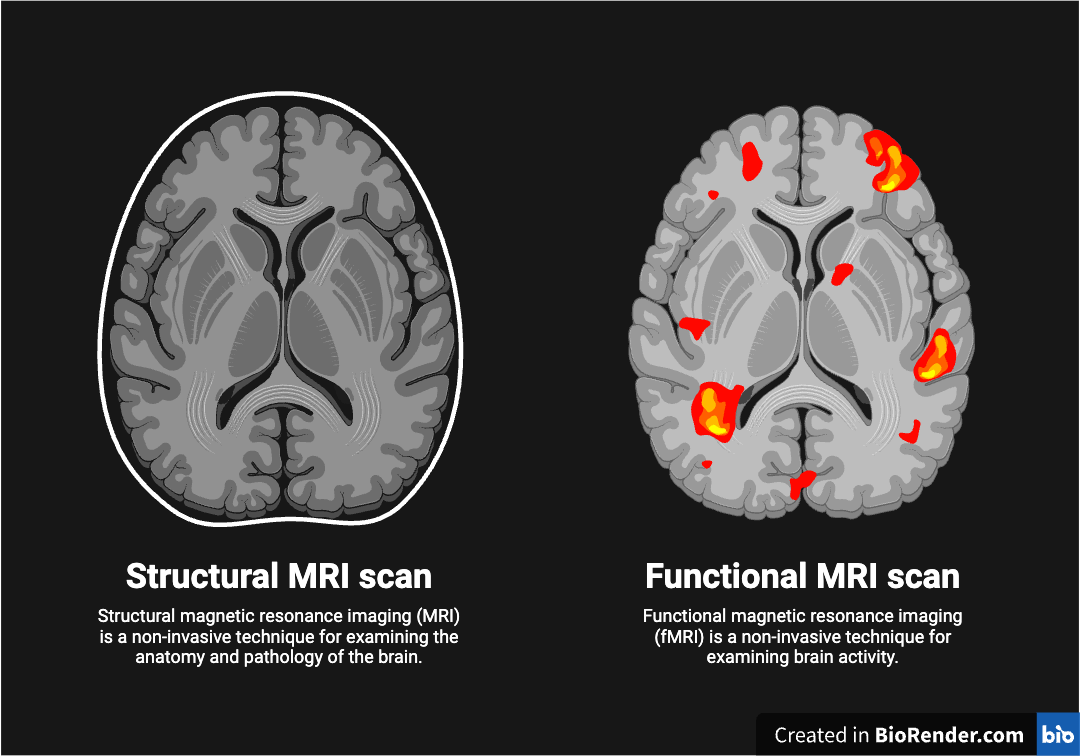
\includegraphics[
    %                         height=3cm,
    %                         trim={595 210 80 70},
    %                         clip
    %                     ]{data/smri_fmri.png}
    %                 };
    %                 \node[anchor=west] at (1.5, -4) {
    %                     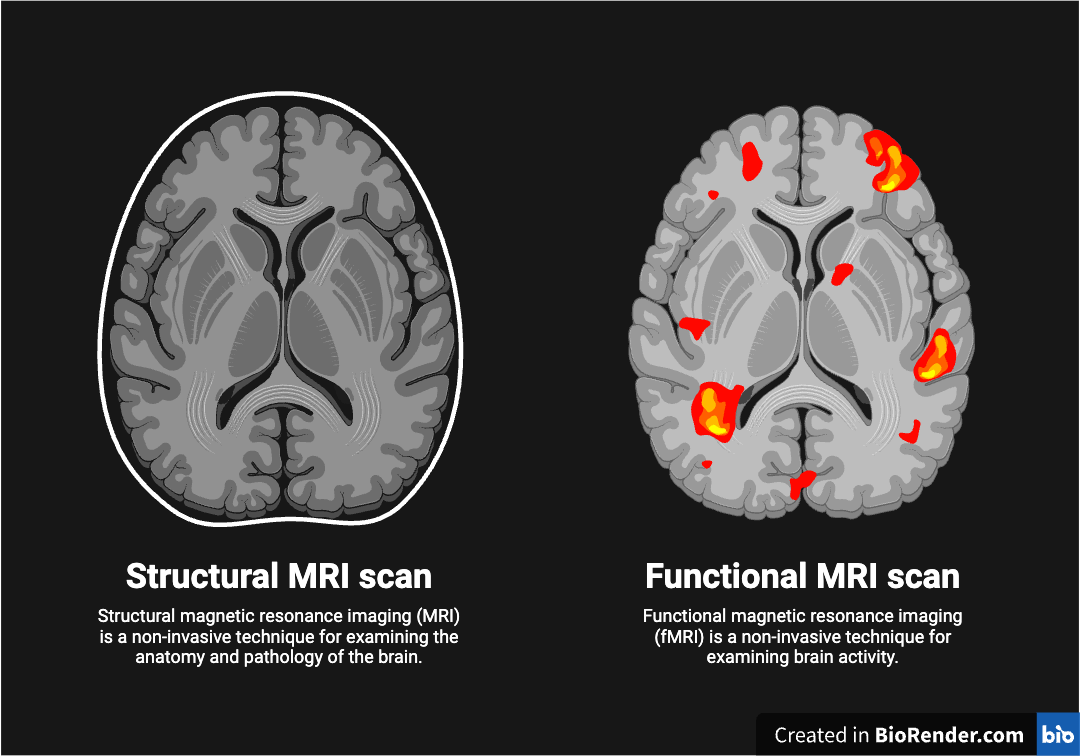
\includegraphics[
    %                         height=3cm,
    %                         trim={75 210 590 70},
    %                         clip
    %                     ]{data/smri_fmri.png}
    %                 };
    %                 \node[anchor=west] at (1.5, -4) {
    %                     \includegraphics[
    %                         height=3cm,
    %                         trim={595 210 80 70},
    %                         clip
    %                     ]{data/smri_fmri.png}
    %                 };
    %                 \node[anchor=west] at (2, -4.5) {
    %                     \includegraphics[
    %                         height=3cm,
    %                         trim={75 210 590 70},
    %                         clip
    %                     ]{data/smri_fmri.png}
    %                 };

    %                 \node[anchor=west] (last) at (2, -4.5) {
    %                     \includegraphics[
    %                         height=3cm,
    %                         trim={595 210 80 70},
    %                         clip
    %                     ]{data/smri_fmri.png}
    %                 };

    %                 \draw[-stealth] ($ (first.north east) + (0.5, -0.13) $) -- ($ (last.north east) + (0.5, -0.13) $) node[midway, above, rotate=315] {time};
    %             }

    %             \only<4>{
    %                 \node[inner sep=0pt, draw=black] at (7.6, -3.2) {
    %                     \includegraphics[
    %                         width=5cm,
    %                         trim={0 0 150 0},
    %                         clip
    %                     ]{data/rest_task.jpeg}
    %                 };
    %                 \node[font=\tiny, anchor=south,align=center, inner sep=1pt] (ms-citation) at (5, -7.65) {
    %                     Branco, P., Seixas, D., Deprez, S., Kovacs, S., Peeters, R., Castro, S. L., \& Sunaert, S. (2016). Resting-state functional magnetic\\resonance imaging for language preoperative planning. Frontiers in human neuroscience, 10, 11
    %                 };
    %             };
    %             \only<5>{
    %                 \node[] at (7.6, -3.6) {
    %                     \usebox{\fmristudies}
    %                 };
    %             }
    %             \only<6>{
    %                 \node[] at (5, -3.2) {
    %                     \usebox{\mddfmri}
    %                 };
    %             }
    %             \only<7-11>{
    %                 \node[font=\tiny, anchor=south,align=center, inner sep=1pt] (ms-citation) at (5, -7.65) {
    %                     Drysdale, A. T., Grosenick, L., Downar, J., Dunlop, K., Mansouri, F., Meng, Y., ... \& Liston, C. (2017). Resting-state connectivity\\biomarkers define neurophysiological subtypes of depression. Nature medicine, 23(1), 28-38
    %                 };
    %                 \only<7>{
    %                     \node[inner sep=0pt, draw=black] at (5, -3.6) {
    %                         \includegraphics[width=5.5cm]{data/mdd_biotypes_overview.jpeg}
    %                     };
    %                 }
    %                 \only<8>{
    %                     \node[inner sep=0pt, draw=black] at (5, -3.6) {
    %                         \includegraphics[
    %                             width=8cm,
    %                             trim={0 6.9cm 0 5.7cm},
    %                             clip
    %                         ]{data/mdd_biotypes_features.jpeg}
    %                     };
    %                 }
    %                 \only<9>{
    %                     \node[inner sep=0pt, draw=black] at (5, -3.6) {
    %                         \includegraphics[
    %                             width=9cm,
    %                             trim={0 0 0 13cm},
    %                             clip
    %                         ]{data/mdd_biotypes_replication.jpeg}
    %                     };
    %                 }
    %                 \only<10,11>{
    %                     \node[inner sep=0pt, draw=black] at (2.5, -3.6) {
    %                         \includegraphics[
    %                             height=2cm,
    %                             trim={0 13.3cm 7.2cm 0},
    %                             clip
    %                         ]{data/mdd_biotypes_treatment.jpeg}
    %                     };
    %                 }
    %                 \only<11>{
    %                     \node[inner sep=0pt, draw=black] at (7.5, -3.6) {
    %                         \includegraphics[
    %                             height=2.8cm,
    %                             trim={0 0 0 9.6cm},
    %                             clip
    %                         ]{data/mdd_biotypes_treatment.jpeg}
    %                     };
    %                 }
    %             }
    %             \onslide<12->{
    %                 \node[font=\tiny, anchor=south,align=center, inner sep=1pt] (ms-citation) at (5, -7.65) {
    %                     Dinga, R., Schmaal, L., Penninx, B. W., van Tol, M. J., Veltman, D. J., van Velzen, L., ... \& Marquand, A. F. (2019). Evaluating the evidence\\for biotypes of depression: Methodological replication and extension of. NeuroImage: Clinical, 22, 101796
    %                 };
    %                 \only<12>{
    %                     \node[inner sep=0pt, draw=black] at (5, -3.2) {
    %                         \includegraphics[width=8cm]{data/dinga_pipeline.jpg}
    %                     };
    %                 }
    %                 \only<13>{
    %                     \node[inner sep=0pt, draw=black] at (5, -3.2) {
    %                         \includegraphics[width=5cm]{data/dinga_results.jpg}
    %                     };
    %                 }
    %             }
    %         \end{tikzpicture}
    %     }
    %     \only<14>{
    %         \begin{itemize}
    %             \setlength\itemsep{-0.3em}
    %             \item[\textcolor{gray!50}{\textbullet}] \textcolor{gray!50}{\footnotesize{Non-T1 weighted structural MRI}}
    %             \begin{itemize}
    %                 \setlength\itemsep{-0.4em}
    %                 \item[\textcolor{gray!50}{\textbullet}] \textcolor{gray!50}{\scriptsize{High accuracies for classifying MS and PD (>90\%).}}
    %                 \item[\textcolor{gray!50}{\textbullet}] \textcolor{gray!50}{\scriptsize{T2-weighted images used by Storelli et al. for predicting MS prognosis.}}
    %                 \item[\textcolor{gray!50}{\textbullet}] \textcolor{gray!50}{\scriptsize{T2-weighted images used by Talai et al. for differential diagnosis of PD and PSP-RS.}}
    %             \end{itemize}
    %             \item[\textcolor{gray!50}{\textbullet}] \textcolor{gray!50}{\footnotesize{Diffusion MRI}}
    %             \begin{itemize}
    %                 \setlength\itemsep{-0.4em}
    %                 \item[] \textcolor{gray!50}{\scriptsize{Few prediction studies, mostly for mental disorders with various accuracies (60-100\%) and DEM (80-100\%)}}
    %                 \item[\textcolor{gray!50}{\textbullet}] \textcolor{gray!50}{\scriptsize{Used by Saglam et al. to differentially diagnose SCZ and BP with 80\% accuracy.}}
    %                 \item[\textcolor{gray!50}{\textbullet}] \textcolor{gray!50}{\scriptsize{Used by Sun et al. to predict conversion from MCI to AD with 81\% accuracy.}}
    %             \end{itemize}
    %             \item {\footnotesize Functional MRI}
    %             \begin{itemize}
    %                 \setlength\itemsep{-0.4em}
    %                 \item {\scriptsize Widely used for all conditions, most prominently SCZ and MDD with varying accuracies (60-100\%) and DEM (80-100\%).}
    %                 \item {\scriptsize Used by Drysdale et al. to detect biotypes of MDD that reacted differently to treatment by transcranial magnetic stimulation.}
    %                 \item {\scriptsize However, Dinga et al. failed to replicate their results \textcolor{red}{WHY}.}
    %             \end{itemize}
    %         \end{itemize}

    %     }
    % \end{frame}

    % \newsavebox{\molstudies}
    % \sbox{\molstudies}{%
    %     \modalityplot{molecular_studies.csv}{{2014, 2018, 2022}}{2011}{2023}{
    %         \node[circle,anchor=south west, draw=pd, fill=pd!75,inner sep=2pt,label=right:{\footnotesize{PD (12)}}] at (axis cs: 2024, 51) {};
    %         \node[circle,anchor=south west, draw=dem, fill=dem!75,inner sep=2pt,label=right:{\footnotesize{DEM (23)}}] at (axis cs: 2024, 56) {};
    %     }
    % }

    % \newsavebox{\moldem}
    % \sbox{\moldem}{%
    %     \disordermodalityplot{DEM}{PET}{molecular_studies.csv}{92.66}{2900}{dem}{2900}
    % }

    % \newsavebox{\molpd}
    % \sbox{\molpd}{%
    %     \disordermodalityplot{PD}{SPECT}{molecular_studies.csv}{92.02}{1650}{pd}{1650}
    % }

    % \newsavebox{\cascade}
    % \sbox{\cascade}{%
    %     \begin{tikzpicture}
    %         \begin{axis}[
    %             ymin=0, ymax=1,
    %             xmin=-15,
    %             xmax=35,
    %             height=8cm,
    %             width=10cm
    %         ]
    %         \addplot[
    %             domain=-15:35,
    %             samples=100,
    %             smooth,
    %             color=blue
    %         ] {1/(1+exp(-0.5*x))}; % First sigmoid

    %         \addplot[
    %             domain=-15:35,
    %             samples=100,
    %             smooth,
    %             color=red
    %         ] {1/(1+exp(-0.5*(x-6)))}; % Shifted right by 6

    %         \addplot[
    %             domain=-15:35,
    %             samples=100,
    %             smooth,
    %             color=green
    %         ] {1/(1+exp(-0.5*(x-12)))}; % Shifted right by 12

    %         \addplot[
    %             domain=-15:35,
    %             samples=100,
    %             smooth,
    %             color=orange
    %         ] {1/(1+exp(-0.5*(x-18)))}; % Shifted right by 18
    %         \end{axis}
    %     \end{tikzpicture}
    % }

    % \begin{frame}[t]{Molecular imaging (PET/SPECT)}
    %     \only<1-22>{
    %         \begin{tikzpicture}
    %             \node[draw=black] at (0, 0) {};
    %             \node[draw=black] at (10, -7) {};

    %             \only<1-4>{
    %                 \node[] at (2, -3.5) {
    %                     \includegraphics[
    %                         width=2.5cm,
    %                         trim={4cm 3cm 60cm 6cm},
    %                         clip
    %                     ]{data/fdg_t1.png}
    %                 };
    %             }
    %             \only<3-4>{
    %                 \node[] at (2, -3.5) {
    %                     \includegraphics[
    %                         width=2.5cm,
    %                         trim={60cm 3cm 4cm 6cm},
    %                         clip
    %                     ]{data/fdg_t1.png}
    %                 };
    %             }
    %             \only<4>{
    %                 \node[] at (7.2, -3.6) {
    %                     \usebox{\molstudies}
    %                 };
    %             }
    %             \only<5>{
    %                 \node[] at (5, -3.2) {
    %                     Explanation of PET
    %                 };
    %             }
    %             \only<6>{
    %                 \node[] at (5, -3.6) {
    %                     \usebox{\moldem}
    %                 };
    %             }
    %             \only<7-15>{
    %                 \only<7>{
    %                     \node[] at (5, -3.75) {
    %                         \usebox{\cascade}
    %                     };
    %                 }
    %                 \only<8-10>{
    %                     \node[font=\tiny, anchor=south,align=center, inner sep=1pt] (ms-citation) at (5, -7.5) {
    %                         Chételat, G., Arbizu, J., Barthel, H., Garibotto, V., Lammertsma, A. A., Law, I., ... \& Drzezga, A. (2021). Finding our way through the\\labyrinth of dementia biomarkers. European journal of nuclear medicine and molecular imaging, 48, 2320-2324
    %                     };
    %                 }
    %                 \only<8>{
    %                     \node[anchor=west] at (0.4, -3.2) {
    %                         \includegraphics[
    %                             height=5cm,
    %                             trim={0 0 23.6cm 0},
    %                             clip
    %                         ]{data/AD_pet_types.png}
    %                     };
    %                 }
    %                 \only<9>{
    %                     \node[anchor=west] at (0.4, -3.2) {
    %                         \includegraphics[
    %                             height=5cm,
    %                             trim={0 0 15.9cm 0},
    %                             clip
    %                         ]{data/AD_pet_types.png}
    %                     };
    %                 }
    %                 \only<10>{
    %                     \node[anchor=west] at (0.4, -3.2) {
    %                         \includegraphics[
    %                             height=5cm,
    %                             trim={0 0 7.85cm 0},
    %                             clip
    %                         ]{data/AD_pet_types.png}
    %                     };
    %                 }
    %                 \only<11>{
    %                     \node[anchor=west] at (0.4, -3.2) {
    %                         \includegraphics[height=5cm]{data/AD_pet_types.png}
    %                     };
    %                 }
    %                 \only<12>{
    %                     \node[font=\scriptsize\itshape, align=left] at (5.2, -3.5) {
    %                         "It is necessary to separate syndrome (clinically identified impairment) from biology\\(etiology)\\
    %                         \\[-0.2cm]
    %                         AD is defined by its biology with the following implications\\
    %                         \\[-0.2cm]
    %                         The disease is first evident with the appearance of β-amyloid plaques, and later\\neocortical tau tangles, while people are asymptomatic. Pathophysiologic mechanisms\\involved with processing and clearance of protein fragments may be involved very early\\in the disease process, but these are not yet well understood.\\
    %                         \\[-0.2cm]
    %                         In living people the disease is diagnosed by disease specific core biomarkers\\
    %                         \\[-0.2cm]
    %                         Unimpaired individuals with abnormal biomarker testing are at risk for symptoms due to\\AD.\\
    %                         \\[-0.2cm]
    %                         They are not at risk for a disease they already have.\\
    %                         \\[-0.2cm]
    %                         Symptoms are a result of the disease process and are not necessary to diagnose AD\\
    %                         \\[-0.2cm]
    %                         AD exists on a continuum not as discrete clinically defined entities\\
    %                         \\[-0.2cm]
    %                         Clinical syndromes commonly seen with AD may also be caused by disorders other than\\AD and therefore clinical presentation alone is not diagnostic of AD\\
    %                         \\[-0.2cm]
    %                         The same AD biology may result in different phenotypic presentations"\\
    %                     };

    %                 }
    %                 \only<13-15>{
    %                     \node[font=\tiny, anchor=south,align=center, inner sep=1pt] (ms-citation) at (5, -7.5) {
    %                         Perovnik, M., Vo, A., Nguyen, N., Jamšek, J., Rus, T., Tang, C. C., ... \& Eidelberg, D. (2022). Automated differential diagnosis\\of dementia syndromes using FDG PET and machine learning. Frontiers in Aging Neuroscience, 14, 1005731
    %                     };
    %                     \only<13>{
    %                         \node[inner sep=0pt, draw=black] at (5, -3.25) {
    %                             \includegraphics[width=7cm]{data/PET_AD_pipeline.jpeg}
    %                         };
    %                     }
    %                     \only<14,15>{
    %                         \node[font=\scriptsize, label=below:\footnotesize{Model predicted diagnosis (86\%)}] at (5, -1.5) {
    %                             \begin{tabular}{r|c|c|c|c|}
    %                                 &\textbf{AD}&\textbf{DLB}&\textbf{FTD}&\textbf{NC}\\
    %                                 \hline
    %                                 \textbf{AD}&53&7&&3\\
    %                                 \hline
    %                                 \textbf{DLB}&9&65&1&4\\
    %                                 \hline
    %                                 \textbf{FTD}&&1&21&1\\
    %                                 \hline
    %                                 \textbf{NC}&2&&&39\\
    %                                 \hline
    %                             \end{tabular}
    %                         };
    %                         \only<15>{
    %                             \node[font=\scriptsize, label=below:\footnotesize{Human predicted diagnosis (78\%)}] at (5, -4.5) {
    %                                 \begin{tabular}{r|c|c|c|c|c|}
    %                                     &\textbf{AD}&\textbf{DLB}&\textbf{FTD}&\textbf{Other}&\textbf{NC}\\
    %                                     \hline
    %                                     \textbf{AD}&50&4&&8&1\\
    %                                     \hline
    %                                     \textbf{DLB}&5&54&&19&1\\
    %                                     \hline
    %                                     \textbf{FTD}&3&&16&24&\\
    %                                     \hline
    %                                     \textbf{Other}&&&&&\\
    %                                     \hline
    %                                     \textbf{NC}&&&&&41\\
    %                                     \hline
    %                                 \end{tabular}
    %                             };
    %                         }
    %                     }
    %                 }
    %             }
    %             \only<16-22>{
    %                 \only<16>{
    %                     \node[] at (7.6, -3.2) {
    %                         \usebox{\molpd}
    %                     };
    %                 }
    %                 \only<17,18>{
    %                     \node[inner sep=0pt, outer sep=0pt] (pet) at (5, -2.2) {
    %                         \includegraphics[
    %                             width=3cm,
    %                             trim={0 0 5.5cm 0},
    %                             clip
    %                         ]{data/PD_PET.jpg}
    %                     };
    %                     \node[font=\tiny, anchor=south,align=center, inner sep=1pt] (ms-citation) at (5, -7.5) {
    %                         Pagano, G., Niccolini, F., \& Politis, M. (2016). Imaging in Parkinson’s disease. Clinical Medicine, 16(4), 371
    %                     };

    %                 }
    %                 \only<18>{
    %                     \node[inner sep=0pt, anchor=north, outer sep=0pt] at ($ (pet.south) + (0, 0.05) $){
    %                         \includegraphics[
    %                             width=3cm,
    %                             trim={3.83cm 0 3.5cm 0},
    %                             clip
    %                         ]{data/PD_SPECT.jpg}
    %                     };
    %                 }
    %                 \only<19>{
    %                     \node[] at (5, -3.5) {
    %                         Explanation of SPECT
    %                     };
    %                 }
    %                 \onslide<20->{
    %                     \node[font=\tiny, anchor=south,align=center, inner sep=1pt] (ms-citation) at (5, -7.5) {
    %                         Adams, M. P., Rahmim, A., \& Tang, J. (2021). Improved motor outcome prediction in Parkinson's disease\\applying deep learning to DaTscan SPECT images. Computers in Biology and Medicine, 132, 104312
    %                     };
    %                     \only<20>{
    %                         \node[inner sep=0pt, draw=black] at (5, -3.75) {
    %                             \includegraphics[width=4.5cm]{data/PD_SPECT_images.jpg}
    %                         };
    %                     }
    %                     \only<21>{
    %                         \node[inner sep=0pt, draw=black] at (5, -3.75) {
    %                             \includegraphics[width=7cm]{data/PD_SPECT_model.jpg}
    %                         };
    %                     }
    %                     \only<22>{
    %                         \node[inner sep=0pt, draw=black] at (5, -3.75) {
    %                             \includegraphics[width=8cm]{data/PD_SPECT_results.jpg}
    %                         };
    %                     }
    %                 }
    %             }
    %         \end{tikzpicture}
    %     }
    %     \only<23>{
    %         \begin{itemize}[itemsep=-0.3em]
    %             \item[\textcolor{gray!50}{\textbullet}] {\footnotesize \textcolor{gray!50}{Non-T1 weighted structural MRI}}
    %             \begin{itemize}[itemsep=-0.3em]
    %                 \vspace{-0.4em}
    %                 \item[\textcolor{gray!50}{\textbullet}] {\scriptsize \textcolor{gray!50}{\setlength{\baselineskip}{10pt}High accuracies for classifying MS and PD (>90\%).}}
    %                 \item[\textcolor{gray!50}{\textbullet}] {\scriptsize \textcolor{gray!50}{T2-weighted images used by Storelli et al. for predicting MS prognosis.}}
    %                 \item[\textcolor{gray!50}{\textbullet}] {\scriptsize \textcolor{gray!50}{T2-weighted images used by Talai et al. for differential diagnosis of PD and PSP-RS.}}
    %             \end{itemize}
    %             \item[\textcolor{gray!50}{\textbullet}] {\footnotesize \textcolor{gray!50}{Diffusion MRI}}
    %             \begin{itemize}[itemsep=-0.3em]
    %                 \vspace{-0.4em}
    %                 \item[\textcolor{gray!50}{\textbullet}] {\scriptsize \textcolor{gray!50}{Few prediction studies, mostly for mental disorders with various accuracies (60-100\%) and DEM (80-100\%)}}
    %                 \item[\textcolor{gray!50}{\textbullet}] {\scriptsize \textcolor{gray!50}{Used by Saglam et al. to differentially diagnose SCZ and BP with 80\% accuracy.}}
    %                 \item[\textcolor{gray!50}{\textbullet}] {\scriptsize \textcolor{gray!50}{Used by Sun et al. to predict conversion from MCI to AD with 81\% accuracy.}}
    %             \end{itemize}
    %             \item[\textcolor{gray!50}{\textbullet}] \textcolor{gray!50}{\footnotesize{Functional MRI}}
    %             \begin{itemize}
    %                 \item[\textcolor{gray!50}{\textbullet}] \textcolor{gray!50}{\scriptsize{Widely used for all conditions, most prominently SCZ and MDD with varying accuracies (60-100\%) and DEM (80-100\%).}}
    %                 \item[\textcolor{gray!50}{\textbullet}] \textcolor{gray!50}{\scriptsize{Used by Drysdale et al. to detect biotypes of MDD that reacted differently to treatment by transcranial magnetic stimulation.}}
    %                 \item[\textcolor{gray!50}{\textbullet}] \textcolor{gray!50}{\scriptsize{However, Dinga et al. failed to replicate their results.}}
    %             \end{itemize}
    %             \item {\footnotesize Molecular imaging}
    %             \begin{itemize}
    %                 \item {\scriptsize Used in a moderate amount of studies predicting PD and DEM with good results (mean accuracy=92\%).}
    %                 \item {\scriptsize PET is excellent for detecting AD-related pathology, and was shown by Pevronik et al. to differentially diagnose DEM above human level. }
    %                 \item {\scriptsize SPECT is excellent for detecting XXX in PD, and was shown by Adams et al. to prognosticate motor function beyond what was done by current motor function alone.}
    %             \end{itemize}
    %         \end{itemize}
    %     }
    % \end{frame}

    % \begin{frame}{Summary}
    %     \begin{itemize}
    %         \setlength\itemsep{-0.3em}
    %         \item \footnotesize{Non-T1 weighted structural MRI}
    %         \begin{itemize}
    %             \item \scriptsize{High accuracies for classifying MS and PD (>90\%).}
    %             \item \scriptsize{T2-weighted images used by Storelli et al. for predicting MS prognosis.}
    %             \item \scriptsize{XXX used by YYY for ZZZ in PD.}
    %         \end{itemize}
    %         \item \footnotesize{Diffusion MRI}
    %         \begin{itemize}
    %             \item \scriptsize{Mostly used in mental disorders with various results (accuracies XX-YY), but also DEM (XX)}
    %             \item \scriptsize{Used by Saglam et al. to differentially diagnose SCZ and BP with 80\% accuracy.}
    %             \item \scriptsize{XXX used by YYY for ZZZ in DEM.}
    %         \end{itemize}
    %         \item \footnotesize{Functional MRI}
    %         \begin{itemize}
    %             \item \scriptsize{Widely used for all disorders, with varying results}
    %             \item \scriptsize{Task-based fMRI used by YYY for ZZZ in SCZ.}
    %             \item \scriptsize{Resting state fMRI used by Segal et al. to make diagnostic predictions at various biological levels.}
    %         \end{itemize}
    %         \item \footnotesize{Molecular imaging}
    %         \begin{itemize}
    %             \item \scriptsize{Mostly used in DEM and PD with high accuracies (~92\%).}
    %             \item \scriptsize{PET used clinically to diagnose Alzheimer's disease.}
    %             \item \scriptsize{SPECT used clinically to XXX Parkinson's disease.}
    %         \end{itemize}
    %     \end{itemize}
    % \end{frame}

    % \section{The future of neuroimaging-based prediction}

    % \newsavebox{\accuracyplots}
    % \sbox{\accuracyplots}{%
    %     \begin{tikzpicture}
    %         \begin{axis}[
    %             boxplot/draw direction = y,
    %             width=10cm,
    %             height=7cm,
    %             xmin=0.4,
    %             xmax=6.6,
    %             ymin=50,
    %             ymax=100,
    %             xtick={1,2,3,4,5,6},
    %             xticklabels={DEM,MS,PD,SCZ,MDD,BP},
    %             ylabel=Accuracy,
    %             axis y line*=left,
    %             xlabel=Diagnosis,
    %             axis x line*=bottom,
    %             clip=false,
    %             xtick style={draw=none},
    %             ymajorgrids=true,
    %             ytick style={draw=none},
    %         ]
    %         % DEM
    %         \addplot[] coordinates { (0.595, 92.5) (1.405, 92.5) };
    %         \addplot[] coordinates { (1.595, 93.4) (2.405, 93.4) };
    %         \addplot[] coordinates { (2.595, 95.15) (3.405, 95.15) };
    %         \addplot[] coordinates { (3.595, 81.8) (4.405, 81.8) };
    %         \addplot[] coordinates { (4.595, 85) (5.405, 85) };
    %         \addplot[] coordinates { (5.595, 68.2) (6.405, 68.2) };
    %         \node[anchor=south] at (axis cs: 1, 92.5) {92.5\%};
    %         \node[anchor=south] at (axis cs:2, 93.4) {93.4\%};
    %         \node[anchor=south] at (axis cs:3, 95.15) {95.15\%};
    %         \node[anchor=south] at (axis cs:4, 81.8) {81.8\%};
    %         \node[anchor=south] at (axis cs:5, 85) {85\%};
    %         \node[anchor=south] at (axis cs:6, 68.2) {68.2\%};
    %         \end{axis}
    %     \end{tikzpicture}
    % }

    % \newsavebox{\boxplots}
    % \sbox{\boxplots}{%
    %     \begin{tikzpicture}
    %         \begin{axis}[
    %             boxplot/draw direction = y,
    %             width=10cm,
    %             height=7cm,
    %             xmin=0.4,
    %             xmax=6.6,
    %             ymin=50,
    %             ymax=100,
    %             xtick={1,2,3,4,5,6},
    %             xticklabels={DEM,MS,PD,SCZ,MDD,BP},
    %             ylabel=Accuracy,
    %             axis y line*=left,
    %             xlabel=Diagnosis,
    %             axis x line*=bottom,
    %             clip=false,
    %             xtick style={draw=none},
    %             ymajorgrids=true,
    %             ytick style={draw=none},
    %         ]
    %         % DEM
    %         \addplot[red] coordinates { (0.595, 92.5) (1.405, 92.5) };
    %         \addplot+[
    %             boxplot prepared={
    %             median=92.5,
    %             upper quartile=97.25,
    %             lower quartile=88.94,
    %             upper whisker=100,
    %             lower whisker=76.46
    %             },
    %             draw=black,
    %             fill=color1,
    %             solid
    %         ] coordinates {};

    %         % MS
    %         \addplot+[
    %             boxplot prepared={
    %             median=93.4,
    %             upper quartile=98.26,
    %             lower quartile=87.9,
    %             upper whisker=100,
    %             lower whisker=72.36
    %             },
    %             draw=black,
    %             fill=color2,
    %             solid
    %         ] coordinates {};

    %         % PD
    %         \addplot+[
    %             boxplot prepared={
    %             median=95.15,
    %             upper quartile=97.07,
    %             lower quartile=89.15,
    %             upper whisker=100,
    %             lower whisker=77.26
    %             },
    %             draw=black,
    %             fill=color3,
    %             solid
    %         ] coordinates {};

    %         % SCZ
    %         \addplot+[
    %             boxplot prepared={
    %             median=81.8,
    %             upper quartile=90.28,
    %             lower quartile=75,
    %             upper whisker=100,
    %             lower whisker=62
    %             },
    %             draw=black,
    %             fill=color4,
    %             solid
    %         ] coordinates {};

    %         % MDD
    %         \addplot+[
    %             boxplot prepared={
    %             median=85,
    %             upper quartile=91.7,
    %             lower quartile=73,
    %             upper whisker=99,
    %             lower whisker=50.55
    %             },
    %             draw=black,
    %             fill=color5,
    %             solid
    %         ] coordinates {};

    %         % BP
    %         \addplot+[
    %             boxplot prepared={
    %             median=68.2,
    %             upper quartile=78.59,
    %             lower quartile=61.03,
    %             upper whisker=100,
    %             lower whisker=55.9
    %             },
    %             draw=black,
    %             fill=color6,
    %             solid
    %         ] coordinates {};
    %         \end{axis}
    %     \end{tikzpicture}
    % }

    % \newsavebox{\sizeplots}
    % \sbox{\sizeplots}{%
    %     \begin{tikzpicture}
    %         \begin{groupplot}[
    %             group style={
    %                 group size=3 by 2,
    %                 horizontal sep=0.25cm,
    %                 group name=plots,
    %                 vertical sep=1.35cm
    %             },
    %             height=3.9cm,
    %             width=4.4cm,
    %             ymin=50,
    %             ymax=100,
    %             ticklabel style = {font=\footnotesize},
    %             xmin=0,
    %             xlabel={\footnotesize{Size}},
    %             x label style={at={(axis description cs:0.5,-0.15)},anchor=north},
    %             y label style={at={(axis description cs:-0.15,.5)},anchor=south},
    %         ]
    %             \nextgroupplot[
    %                 ylabel={\footnotesize{Accuracy}},
    %                 ymajorgrids=true,
    %                 ytick style={draw=none},
    %                 xmax=4700
    %             ]
    %                 \addplot[
    %                     color1,
    %                     only marks,
    %                     opacity=0.5
    %                 ] table [
    %                     x=sample,
    %                     y=accuracy,
    %                     col sep=comma
    %                 ] {data/DEM_accuracy_sample.csv};

    %             \nextgroupplot[
    %                 ymajorticks=false,
    %                 ymajorgrids=true,
    %                 xmax=1600
    %             ]
    %                 \addplot[
    %                     color2,
    %                     only marks,
    %                     opacity=0.5
    %                 ] table [
    %                     x=sample,
    %                     y=accuracy,
    %                     col sep=comma
    %                 ] {data/MS_accuracy_sample.csv};

    %             \nextgroupplot[
    %                 ymajorticks=false,
    %                 ymajorgrids=true,
    %                 xmax=1700
    %             ]
    %                 \addplot[
    %                     color3,
    %                     only marks,
    %                     opacity=0.5
    %                 ] table [
    %                     x=sample,
    %                     y=accuracy,
    %                     col sep=comma
    %                 ] {data/PD_accuracy_sample.csv};

    %             \nextgroupplot[
    %                 ylabel={\footnotesize{Accuracy}},
    %                 ytick style={draw=none},
    %                 ymajorgrids=true,
    %                 xmax=1250
    %             ]
    %                 \addplot[
    %                     color4,
    %                     only marks,
    %                     opacity=0.5
    %                 ] table [
    %                     x=sample,
    %                     y=accuracy,
    %                     col sep=comma
    %                 ] {data/SCZ_accuracy_sample.csv};

    %             \nextgroupplot[
    %                 ymajorticks=false,
    %                 ymajorgrids=true,
    %                 xmax=395
    %             ]
    %                 \addplot[
    %                     color5,
    %                     only marks,
    %                     opacity=0.5
    %                 ] table [
    %                     x=sample,
    %                     y=accuracy,
    %                     col sep=comma
    %                 ] {data/MDD_accuracy_sample.csv};

    %             \nextgroupplot[
    %                 ymajorticks=false,
    %                 ymajorgrids=true,
    %                 xmax=3300
    %             ]
    %                 \addplot[
    %                     color6,
    %                     only marks,
    %                     opacity=0.5
    %                 ] table [
    %                     x=sample,
    %                     y=accuracy,
    %                     col sep=comma
    %                 ] {data/BP_accuracy_sample.csv};
    %             \end{groupplot}
    %         \node[anchor=south] at (plots c1r1.north) {\textbf{\footnotesize{DEM}}};
    %         \node[anchor=south] at (plots c2r1.north) {\textbf{\footnotesize{MS}}};
    %         \node[anchor=south] at (plots c3r1.north) {\textbf{\footnotesize{PD}}};
    %         \node[anchor=south] at (plots c1r2.north) {\textbf{\footnotesize{SCZ}}};
    %         \node[anchor=south] at (plots c2r2.north) {\textbf{\footnotesize{MDD}}};
    %         \node[anchor=south] at (plots c3r2.north) {\textbf{\footnotesize{BP}}};
    %     \end{tikzpicture}
    % }

    % \newsavebox{\trendplots}
    % \sbox{\trendplots}{%
    %     \begin{tikzpicture}
    %         \begin{groupplot}[
    %             group style={
    %                 group size=3 by 2,
    %                 horizontal sep=0.25cm,
    %                 group name=plots,
    %                 vertical sep=1.35cm
    %             },
    %             height=3.9cm,
    %             width=4.4cm,
    %             ymin=50,
    %             ymax=100,
    %             ticklabel style = {font=\footnotesize},
    %             xmin=0,
    %             xlabel={\footnotesize{Size}},
    %             x label style={at={(axis description cs:0.5,-0.15)},anchor=north},
    %             y label style={at={(axis description cs:-0.15,.5)},anchor=south},
    %         ]
    %             \nextgroupplot[
    %                 ylabel={\footnotesize{Accuracy}},
    %                 ymajorgrids=true,
    %                 ytick style={draw=none},
    %                 xmax=4700
    %             ]
    %                 \addplot[
    %                     color1,
    %                     only marks,
    %                     opacity=0.5
    %                 ] table [
    %                     x=sample,
    %                     y=accuracy,
    %                     col sep=comma
    %                 ] {data/DEM_accuracy_sample.csv};
    %                 \addplot[black, thick] coordinates {
    %                     (0, 91.0895) (4700, 91.0895+4500*0.0014)
    %                 };

    %             \nextgroupplot[
    %                 ymajorticks=false,
    %                 ymajorgrids=true,
    %                 xmax=1600
    %             ]
    %                 \addplot[
    %                     color2,
    %                     only marks,
    %                     opacity=0.5
    %                 ] table [
    %                     x=sample,
    %                     y=accuracy,
    %                     col sep=comma
    %                 ] {data/MS_accuracy_sample.csv};
    %                 \addplot[black, thick] coordinates {
    %                     (0, 92.5003) (4500, 92.5003+1600*-0.0039)
    %                 };

    %             \nextgroupplot[
    %                 ymajorticks=false,
    %                 ymajorgrids=true,
    %                 xmax=1700
    %             ]
    %                 \addplot[
    %                     color3,
    %                     only marks,
    %                     opacity=0.5
    %                 ] table [
    %                     x=sample,
    %                     y=accuracy,
    %                     col sep=comma
    %                 ] {data/PD_accuracy_sample.csv};
    %                 \addplot[black, thick] coordinates {
    %                     (0, 92.9322) (1700, 92.9322+1700*-0.0011)
    %                 };

    %             \nextgroupplot[
    %                 ylabel={\footnotesize{Accuracy}},
    %                 ytick style={draw=none},
    %                 ymajorgrids=true,
    %                 xmax=1250
    %             ]
    %                 \addplot[
    %                     color4,
    %                     only marks,
    %                     opacity=0.5
    %                 ] table [
    %                     x=sample,
    %                     y=accuracy,
    %                     col sep=comma
    %                 ] {data/SCZ_accuracy_sample.csv};
    %                 \addplot[black, thick] coordinates {
    %                     (0, 83.2200) (1700, 83.2200+1250*-0.006)
    %                 };

    %             \nextgroupplot[
    %                 ymajorticks=false,
    %                 ymajorgrids=true,
    %                 xmax=395
    %             ]
    %                 \addplot[
    %                     color5,
    %                     only marks,
    %                     opacity=0.5
    %                 ] table [
    %                     x=sample,
    %                     y=accuracy,
    %                     col sep=comma
    %                 ] {data/MDD_accuracy_sample.csv};
    %                 \addplot[black, thick] coordinates {
    %                     (0, 85.7010) (1700, 85.7010+395*-0.055)
    %                 };

    %             \nextgroupplot[
    %                 ymajorticks=false,
    %                 ymajorgrids=true,
    %                 xmax=3300
    %             ]
    %                 \addplot[
    %                     color6,
    %                     only marks,
    %                     opacity=0.5
    %                 ] table [
    %                     x=sample,
    %                     y=accuracy,
    %                     col sep=comma
    %                 ] {data/BP_accuracy_sample.csv};
    %                 \addplot[black, thick] coordinates {
    %                     (0, 73.0650) (3300, 73.0650+3300*-0.0052)
    %                 };
    %             \end{groupplot}
    %         \node[anchor=south] at (plots c1r1.north) {\textbf{\footnotesize{DEM}}};
    %         \node[anchor=south] at (plots c2r1.north) {\textbf{\footnotesize{MS}}};
    %         \node[anchor=south] at (plots c3r1.north) {\textbf{\footnotesize{PD}}};
    %         \node[anchor=south] at (plots c1r2.north) {\textbf{\footnotesize{SCZ}}};
    %         \node[anchor=south] at (plots c2r2.north) {\textbf{\footnotesize{MDD}}};
    %         \node[anchor=south] at (plots c3r2.north) {\textbf{\footnotesize{BP}}};
    %     \end{tikzpicture}
    % }

    % \begin{frame}{Challenges: Predictiveness}
    %     \begin{tikzpicture}
    %         \node[] at (0, 0) {};
    %         \node[] at (10, -7) {};

    %         \only<1>{
    %             \node[] at (5, -3.5) {
    %                 \usebox{\accuracyplots}
    %             };
    %         }
    %         \only<2>{
    %             \node[] at (5, -3.5) {
    %                 \usebox{\boxplots}
    %             };
    %         }
    %         \only<3>{
    %             \node[] at (5, -3.5) {
    %                 \usebox{\sizeplots}
    %             };
    %         }
    %         \only<4>{
    %             \node[] at (5, -3.5) {
    %                 \usebox{\trendplots}
    %             };
    %         }
    %         \onslide<5->{
    %             \node[] at (5, -6.25) {\scriptsize{Matsuo et al., 2019}};
    %             \node[font=\tiny, align=center, anchor=south] at (5, -7.7) {
    %                 Matsuo, K., Harada, K., Fujita, Y., Okamoto, Y., Ota, M., Narita, H., ... \& Watanabe, Y. (2019). Distinctive neuroanatomical\\substrates for depression in bipolar disorder versus major depressive disorder. Cerebral Cortex, 29(1), 202-214
    %             };
    %             \only<5,6>{
    %                 \node[inner sep=0pt, draw=black, anchor=west] at (2, -3) {
    %                     \includegraphics[
    %                         height=6cm
    %                     ]{data/bp_generalization_before.png}
    %                 };
    %             }
    %             \onslide<7->{
    %                 \node[inner sep=0pt, draw=black,anchor=west] at (2, -3) {
    %                     \includegraphics[
    %                         height=6cm
    %                     ]{data/bp_generalization.png}
    %                 };
    %             }
    %             \onslide<6->{
    %                 \node[red] (insample) at (1, -3.66) {88.1\%};
    %                 \draw[-stealth,red,thick] ($ (insample.east) + (0.63, 0) $) -- (insample);
    %             }
    %             \only<8>{
    %                 \node[red] (outofsample) at (9.06, -5.5) {58.3\%};
    %                 \draw[-stealth,red,thick] ($ (outofsample.west) - (0.63, 0) $) -- (outofsample);
    %             }

    %         }
    %     \end{tikzpicture}
    % \end{frame}


    % \begin{frame}{Challenges: Predictive targets}
    %     \begin{tikzpicture}
    %         \node[] at (0, 0) {};
    %         \node[] at (10, -7) {};



    %         \only<1-4>{
    %             \node[] at (5, -5.15) {\scriptsize{Marquand et al., 2016}};
    %             \node[font=\tiny, align=center, anchor=south] at (5, -7.65) {
    %                 Marquand, A. F., Rezek, I., Buitelaar, J., \& Beckmann, C. F. (2016). Understanding heterogeneity in clinical cohorts using normative\\models: beyond case-control studies. Biological psychiatry, 80(7), 552-561
    %             };
    %             \node[inner sep=0pt, anchor=north west] (a) at (1, 0) {
    %                 \includegraphics[width=4cm]{data/marquand_a.png}
    %             };
    %             \only<1>{
    %                 \draw[] (a.north west) -- (a.north east) -- (a.south east) -- (a.south west) -- cycle;
    %             }
    %         }
    %         \onslide<2-4>{
    %             \node[inner sep=0pt, anchor=west] (b) at (a.east) {
    %                 \includegraphics[width=4cm]{data/marquand_b.png}
    %             };
    %             \only<2>{
    %                 \draw[] (a.north west) -- (b.north east) -- (b.south east) -- (a.south west) -- cycle;
    %             };
    %         }
    %         \onslide<3-4>{
    %             \node[inner sep=0pt, anchor=north] (c) at (a.south) {
    %                 \includegraphics[width=4cm]{data/marquand_c.png}
    %             };
    %             \only<3>{
    %                 \draw[] (a.north west) -- (b.north east) -- (b.south east) -- (b.south west) -- (c.south east) -- (c.south west) -- cycle;
    %             };
    %         }
    %         \only<4>{
    %             \node[inner sep=0pt, anchor=north] (d) at (b.south) {
    %                 \includegraphics[width=4cm]{data/marquand_d.png}
    %             };
    %             \draw[] (a.north west) -- (b.north east) -- (d.south east) -- (c.south west) -- cycle;

    %         }
    %         \only<5>{
    %             \node[] at (5, -3.5) {
    %                 Diagnostic labels vs prognosis, treatment, differential
    %             };
    %         }
    %         \only<6>{
    %             \node[draw=black, inner sep=0pt, label=below:{\scriptsize{Vogel \& Black (2024)}}] at (5, -3.5) {
    %                 \includegraphics[width=4cm]{data/transdiagnostic.png}
    %             };
    %             \node[font=\tiny, anchor=south,align=center, inner sep=1pt] (psych-citation) at (5, -7.65) {
    %                 Vogel, A. C., \& Black, K. J. (2024). Brain Imaging in Routine Psychiatric Practice. Missouri Medicine, 121(1), 37
    %             };
    %         }
    %     \end{tikzpicture}
    % \end{frame}

    % \newsavebox{\nezer}
    % \sbox{\nezer}{%
    %     \begin{tikzpicture}
    %         \begin{axis}[
    %             height=6cm,
    %             width=8cm,
    %             xtick={1,2,3,4,5,6,7,8,9},
    %             xticklabels={H7,H8,H9,H2,H3,H4,H6,H1,H5},
    %             ymin=0,
    %             ymax=1,
    %             xtick pos=left,
    %             ytick pos=bottom,
    %             x tick style={draw=none},
    %             xlabel=Hypothesis,
    %             ylabel style={align=center},
    %             ylabel={Fraction of teams reporting\\a significant result}
    %         ]
    %             \addplot[
    %                 only marks,
    %                 mark=*,
    %                 mark options={
    %                     draw=black,
    %                     fill=color1,
    %                     opacity=0.8
    %                 },
    %                 mark size=2.5pt,
    %                 error bars/.cd,
    %                 y dir=both,
    %                 y explicit,
    %             ] table [
    %                 x=id,
    %                 y=fv,
    %                 y error plus expr=\thisrow{fv_95u}-\thisrow{fv},
    %                 y error minus expr=\thisrow{fv}-\thisrow{fv_95l},
    %                 col sep=comma
    %             ] {data/botvinik_nezer.csv};
    %         \end{axis}
    %     \end{tikzpicture}
    % }

    % \begin{frame}{Challenges: Preprocessing and degrees of freedom}
    %     \begin{tikzpicture}
    %         \node[] at (0, 0) {};
    %         \node[] at (10, -7) {};

    %         \only<1>{
    %             \node[inner sep=0pt, draw=black, label=below:{\scriptsize{Nørgaard et al., 2020}}] at (5, -3.5) {
    %                 \includegraphics[width=9cm]{data/nørgaard.jpeg}
    %             };

    %             \node[font=\tiny, align=center, anchor=south] at (5, -7.65) {
    %                 Nørgaard, M., Ganz, M., Svarer, C., Frokjaer, V. G., Greve, D. N., Strother, S. C., \& Knudsen, G. M. (2020). Different\\preprocessing strategies lead to different conclusions: a [11C] DASB-PET reproducibility study. Journal of Cerebral\\Blood Flow \& Metabolism, 40(9), 1902-1911
    %             };
    %         }

    %         \onslide<2->{
    %             \node[label=below:{\scriptsize{Adapted from Botvinik-Nezer et al., 2020}}] at (5, -2.7) {
    %                 \usebox{\nezer}
    %             };

    %             \node[font=\tiny, align=center, anchor=south] at (5, -7.65) {
    %                 Botvinik-Nezer, R., Holzmeister, F., Camerer, C. F., Dreber, A., Huber, J., Johannesson, M., ... \& Rieck, J. R. (2020). Variability\\in the analysis of a single neuroimaging dataset by many teams. Nature, 582(7810), 84-88
    %             };
    %         }
    %         \onslide<3>{
    %             \node[minimum width=9cm, minimum height=6cm,fill=black!2,opacity=0.85] at (5, -2.7) {};
    %             \node[fill=none,align=center] at (5, -3) {\textit{"On average across the 9 hypotheses, 20\% of teams reported}\\ \textit{a result that differed from the majority of teams. Given that}\\ \textit{the maximum possible variation is 50\%, the observed fraction}\\ \textit{of 20\% divergent results thus \textbf{falls midway between complete}}\\ \textit{\textbf{consistency across teams and completely random results},}\\ \textit{demonstrating that analytical choices have a major effect on}\\ \textit{reported results."}};

    %         }
    %     \end{tikzpicture}
    % \end{frame}

    % \begin{frame}{Challenges: Interpretability}
    %     \centering
    %     \begin{tikzpicture}
    %         \node[] at (0, 0) {};
    %         \node[] at (10, -7) {};
    %         \only<1,3-4>{
    %             \only<1>{
    %                 \node[inner sep=0pt] (bert) at (2, -4)  {
    %                     \includegraphics[width=2.5cm]{data/bert_coronal.png}
    %                 };
    %             }
    %             \only<1,3>{
    %                 \node[align=center,draw=gray,fill=gray!20, minimum width=3cm, minimum height=2cm] (model) at (5.5, -4) {Predictive\\model};
    %             }
    %             \only<1>{
    %                 \node[align=center,text depth=0, anchor=west] (patient) at (8.1, -3.6) {Patient};
    %                 \node[align=center,text depth=0, anchor=west] (control) at (8.1, -4.4) {Control};

    %                 \draw[-stealth, thick] (bert) -- (model);
    %                 \draw[-stealth, thick] (model.east) -- (patient.west);
    %                 \draw[-stealth, thick] (model.east) -- (control.west);
    %             }
    %             \only<4>{
    %                 \node[align=center,draw=gray,fill=gray!20, minimum width=3cm, minimum height=2cm] (model) at (5.5, -4) {a+b+c+d};
    %             }
    %         }
    %         \only<2>{
    %             \node[inner sep=0pt, draw=black, label=below:{\scriptsize{Vogel \& Black (2024)}}] at (5, -3.5) {
    %                 \includegraphics[width=10cm]{data/prediction_vs_interpretability.png}
    %             };
    %                 \node[font=\tiny, anchor=south,align=center, inner sep=1pt] (psych-citation) at (5, -7.65) {
    %                     Vogel, A. C., \& Black, K. J. (2024). Brain Imaging in Routine Psychiatric Practice. Missouri Medicine, 121(1), 37
    %                 };
    %         }
    %         \only<5>{
    %             \node[inner sep=0pt, draw=black] at (5, -3.5){
    %                 \includegraphics[width=8cm]{data/martin_explainable.png}
    %             };
    %         }
    %     \end{tikzpicture}
    % \end{frame}

    % \begin{frame}{Opportunities: New modalities}
    %     \only<1>{
    %         DEBBIE
    %     }
    %     \only<2>{
    %         QSM
    %     }
    % \end{frame}

    % \newsavebox{\multimodalyear}
    % \sbox{\multimodalyear}{%
    %     \begin{tikzpicture}
    %         \begin{axis}[
    %             xmin=2005,
    %             xmax=2022,
    %             xtick={2005,2010,2015,2020},
    %             ytick={0, 0.1, 0.2},
    %             yticklabels={0\%, 10\%, 20\%},
    %             xlabel={Year},
    %             ylabel={Fraction of multimodal studies}
    %         ]
    %             \addplot[
    %                 mark=*,
    %                 mark options={fill=color1},
    %                 mark size=3pt
    %             ] table [
    %                 y=multimodal,
    %                 x=year,
    %                 col sep=comma
    %             ] {data/multimodal_years.csv};
    %         \end{axis}
    %     \end{tikzpicture}
    % }

    % \newsavebox{\multimodalpubmed}
    % \sbox{\multimodalpubmed}{%
    %     \begin{tikzpicture}
    %         \begin{axis}[
    %             xmin=1990,
    %             xmax=2024,
    %             xtick={1990, 2000, 2010, 2020},
    %             xticklabels={1990, 2000, 2010, 2020},
    %             xlabel={Year},
    %             ylabel={Number of studies},
    %             width=9cm,
    %             height=6cm
    %         ]
    %             \addplot[
    %                 mark=*,
    %                 mark options={fill=color1},
    %                 mark size=2pt
    %             ] table [
    %                 y=Count,
    %                 x=Year,
    %                 col sep=comma
    %             ] {data/pubmed_multimodal.csv};
    %         \end{axis}
    %     \end{tikzpicture}
    % }

    % \begin{frame}{Opportunities: Multimodality}
    %     \begin{tikzpicture}
    %         \node[] at (0, 0) {};
    %         \node[] at (10, -7) {};

    %         \only<1-2>{
    %             \node[inner sep=0pt] (bert) at (2, -3.5)  {
    %                 \includegraphics[width=1.5cm]{data/t1.jpg}
    %             };

    %             \node[align=center,draw=gray,fill=gray!20, minimum width=2.5cm, minimum height=1.5cm] (model) at (5.5, -3.5) {Predictive\\model};

    %             \node[align=center,text depth=0, anchor=west] (patient) at (8.1, -3.1) {Patient};
    %             \node[align=center,text depth=0, anchor=west] (control) at (8.1, -3.9) {Control};

    %             \draw[-stealth, thick] (bert) -- (model);
    %             \draw[-stealth, thick] (model.east) -- (patient.west);
    %             \draw[-stealth, thick] (model.east) -- (control.west);

    %             \only<2>{
    %                 \node[inner sep=0pt] (t2) at (2, -1.5)  {
    %                     \includegraphics[width=1.5cm]{data/t2.jpg}
    %                 };
    %                 \node[inner sep=0pt] (flair) at (2, -5.5)  {
    %                     \includegraphics[width=1.5cm]{data/flair.jpg}
    %                 };

    %                 \draw[-stealth, thick] (t2) -- (model.west);
    %                 \draw[-stealth, thick] (flair) -- (model.west);
    %             }
    %         }

    %         \only<3>{
    %             \node[] at (5, -3.5) {
    %                 \usebox{\multimodalpubmed}
    %             };
    %             \node[font=\tiny, align=center, anchor=south] at (5, -7.75) {
    %                 \scriptsize{Pubmed search: multimodal[Title] AND (neuroimaging[Title] or MRI[Title])}
    %             };
    %         }
    %     \end{tikzpicture}
    % \end{frame}

    % \begin{frame}{Opportunities: Larger datasets}
    %     \centering
    %     \begin{tikzpicture}
    %         \begin{axis}[
    %             xmin=1995,
    %             xmax=2023,
    %             ymin=0,
    %             xlabel=Year,
    %             ylabel={Sample size},
    %             set layers,
    %             mark layer=axis tick labels
    %         ]
    %             \addplot[
    %                 only marks,
    %                 mark=*,
    %                 mark options={fill=color4},
    %                 mark size=3pt,
    %                 opacity=0.5
    %             ] table [
    %                 col sep=comma,
    %                 x=year,
    %                 y=sample
    %             ] {data/samples_per_year.csv};
    %             \addplot[
    %                 very thick
    %             ] coordinates {
    %                 (0, -54286)
    %                 (2024, -54286+27*2024)
    %             };
    %         \end{axis}
    %     \end{tikzpicture}
    % \end{frame}

    % \begin{frame}{Opportunities: Better methods}
    %     \centering
    %     \begin{tikzpicture}
    %         \begin{axis}[
    %             xmin=1995,
    %             xmax=2023,
    %             ymin=0,
    %             xlabel=Year,
    %             ylabel={Sample size},
    %             set layers,
    %             mark layer=axis tick labels
    %         ]
    %             \addplot[
    %                 only marks,
    %                 mark=*,
    %                 mark options={fill=color1},
    %                 mark size=3pt,
    %                 opacity=0.5
    %             ] table [
    %                 col sep=comma,
    %                 x=year,
    %                 y=accuracy
    %             ] {data/ML_accuracies.csv};

    %             \addplot[
    %                 only marks,
    %                 mark=*,
    %                 mark options={fill=color7},
    %                 mark size=3pt,
    %                 opacity=0.5
    %             ] table [
    %                 col sep=comma,
    %                 x=year,
    %                 y=accuracy
    %             ] {data/DL_accuracies.csv};
    %             \only<2>{
    %                 \addplot[
    %                     color1,
    %                     very thick
    %                 ] coordinates {
    %                     (0, 200)
    %                     (2024,200-0.059*2024)
    %                 };

    %                 \addplot[
    %                     color7,
    %                     very thick
    %                 ] coordinates {
    %                     (2005, -1251+0.665*2005)
    %                     (2024, -1251+0.665*2024)
    %                 };
    %             }
    %         \end{axis}
    %     \end{tikzpicture}
    % \end{frame}
\end{document}
